\chapterimage{Fig/Chapter5/cover_ch5.png}


\chapter{Towards measuring Tan's contact in 1D gases}

For the last chapter of this thesis, we will depart from the main line set by the \kmk correlations of the quantum depletion and shift our attention to a different topic that exploits another feature of the single-atom resolution of our experiment. While we have used it so far to look for correlations between individual particles, another strong advantage of our apparatus is the possibility to detect very low densities signals inaccessible with optical measurements. An example of such a signal is the $k^{-4}$ tails in the momentum density of 1D gases, also known as Tan's contact \cite{tan2008large}. 

As we will see in the first section of this chapter, Tan's contact is a fascinating and promising universal quantity that can be used to characterize many different systems, especially 1D gases, in level of details inaccessible with more common experimental techniques. We will then quickly summarize the main points of the theoretical work \cite{yao2018tan} on which we will rely to interpret our experimental data. We will next explain how 1D physics can be effectively implemented with our experimental apparatus and detail the procedure used to measure Tan's contact, before discussing the first preliminary results.


\section{Tan's contact}

\subsection{Definition from the large momentum tails}

To understand what Tan's contact is, we consider two atoms with contact interactions in the ultracold regime in 1D. The two-body wave-function then only depends from the inter-particle distance $r$ and the $s$-wave scattering length $a_s$ \cite{viverit2004momentum}:

\begin{equation}
    \psi(r) = - \frac{r}{a_s} \, e^{-r/a_s}
\end{equation}

\noindent The Fourier transform of this expression is rather easy to compute and writes:

\begin{equation}
    \tilde{\psi}(k) = \int_0^\infty \psi(r) \, e^{2 \pi i k r} \, dr \propto \frac{1}{(i 2 \pi k - 1/a_s)^2}
\end{equation}

\noindent from which we obtain the momentum density:

\begin{equation}
     \rho(k) = |\tilde{\psi}(k) |^2 \propto \frac{1}{2(2 \pi k a_s)^4 - 2(2 \pi k a_s)^2 +1}
\end{equation}

\noindent Interestingly, if we look at the asymptotic behavior at large $k$ we find that:

\begin{equation}
    \rho(k) \underrel{k \to \infty} \to \frac{1}{k^4}
    \label{eq:kmf_scaling}
\end{equation}

\noindent The presence of contact interactions translates into a $\kmf$ scaling of the momentum distribution at large $k$. Importantly, this signature holds for higher dimensions, independently of temperature, interaction strength or quantum statistics making it a \textbf{universal relation}. From equation \ref{eq:kmf_scaling}, we define the Tan's Contact $C$ as:

\begin{equation}
    C = \lim_{k \to \infty} k^4 \rho(k)
\end{equation}

Importantly, we will take in this chapter the convention:

\begin{equation}
    \int \frac{d k}{2 \pi} \rho(k)= \NBEC
\end{equation}

\noindent where $\NBEC$ is the total number of atoms, with the notable addition of the factor $1/2 \pi$ to match the definition of the theoretical work \cite{yao2018tan} to which we will compare the experimental data.  

\subsection{Connection to thermodynamic quantities}

While the $\kmf$ scaling is universal, the value of $C$ depends on the physical characteristics of the system such as the number of particles, temperature, dimension etc. and thus contains meaningful information that would otherwise be hard to measure with standard experimental techniques. This was first theorized by Shina Tan in 2008 \cite{tan2008large} who showed that $C$ is a thermodynamic quantity revealing how the total energy of a two component Fermi gas changes when adiabatically tuning the inverse scattering length $a_s$:

\begin{equation}
    -\frac{d E}{d(1 / a_s)}=\frac{h^{2} C}{2 \pi m}
\end{equation}

\noindent This result is known as Tan's adiabatic sweep theorem and can be adapted to the 1D bosonic case \cite{barth2011tan} to obtain:

\begin{equation}
    C=\left.\frac{4 m}{\hbar^{2}} \frac{\partial \Omega}{\partial a_{1 D}}\right|_{T, \mu}
\end{equation}

\noindent with $\Omega$ the grand potential and $a_{\rm{1D}}$ the 1D scattering length whose expression will be discussed later. This result can also be rewritten \cite{yao:tel-03065015} to include the interaction energy of the system $\mean{H_{\rm{int}}}$ that we have often encountered throughout this thesis and that is usually hard to measure separately from the total energy:

\begin{equation}
    C=\frac{2 g_{\rm{1D}} m^{2}}{\hbar^{4}}\left\langle H_{\text {int }}\right\rangle
    \label{eq:C_with_int}
\end{equation}

\noindent with $g_{\rm{1D}}$ the 1D coupling constant that is defined from the 1D scattering length by \cite{olshanii1998atomic}:

\begin{equation}
    g_{\rm{1D}}=-\frac{2 \hbar^2}{m a_{\rm{1D}}}
\end{equation}

\subsection{Characterization of 1D Lieb-Liniger regimes}

Another significant motivation to measure Tan's contact is to characterize the different regimes of Lieb-Liniger 1D systems of interacting bosons as a function of temperature and of the strength of the interactions. Tan's contact is indeed particularly suited to study the Lieb-Liniger model \cite{lieb1963exact} as it revolves around the approximation that the interactions between the atoms are repulsive, contact interactions:

\begin{equation}
    H = \sum_j \left[ - \frac{ \hbar^2}{2m} \frac{\partial^2}{\partial^2 {x_j}^2} + V(x_j) \right] + g_{\rm{1D}} \sum_{j<l} \delta(x_j - x_l) 
    \label{eq:lieb_liniger}
\end{equation}

\noindent with $V$ an external trapping potential. 


These different regimes have been widely investigated \cite{petrov2000regimes} and are illustrated on the state diagram of Fig.\ref{fig:1D_diagram}. The lower right part of the diagram corresponds to the strongly interacting or Tonks-Girardeau regime where the repulsive interactions are so strong that they mimic the Pauli exclusion principle for fermions. The gas is then said to fermionize. As the strength of the interactions decreases, the gas progressively goes to a weakly-interacting quasi-condensate phase characterized by suppressed density fluctuations but fluctuating phase, contrary to the true condensate. The weakly-degenerate ideal bosons region refers to the region where the effect of interactions are negligible compared to temperature. 

The main difficulty to experimentally characterize those regimes resides in the fact that most quantities show a smooth and monotonic behavior when crossing the transition points between the different regimes. This motivated theoretical studies of the dependency of the Tan's contact with the strength of interactions and temperature to determine if $C$ can be used as a probe to characterize these different regimes. Previous works have conducted such studies for homogeneous bosons at finite temperature \cite{kheruntsyan2003pair,kormos2009expectation}, trapped bosons at zero temperature \cite{minguzzi2002high,olshanii2003short} or for the trapped finite temperature Tonks-Girardeau regime \cite{vignolo2013universal}. They were recently completed by \cite{yao2018tan}, characterizing trapped Lieb-Liniger bosons for arbitrary values of the temperature and the interaction parameter.

There have been many experiments aiming at measuring Tan's contact in strongly interacting systems for both bosons and fermions, using a variety of methods such as RF spectroscopy \cite{wild2012measurements,sagi2012measurement}, Ramsey interferometry \cite{fletcher2017two,zou1991violation}, structure factor measurement with Bragg spectroscopy \cite{kuhnle2010universal} or measurements of the momentum distribution \cite{stewart2010verification,luciuk2016evidence}. One of the main experimental difficulties for measuring Tan's contact from the momentum density $\rho(k)$ when the gas is not strongly interacting comes from the fact that the high momentum $\kmf$ tails correspond to very low density values that are hard to detect with classic optical imaging techniques. This problem is however solved with the $\He$ detector thanks to his large dynamic momentum range. Interestingly, our experimental apparatus can be adapted to study 1D physics by transforming our 3D optical lattice into a 2D one as we will see in \ref{sec:1D_exp}, making it a good candidate to verify the predictions of \cite{yao2018tan}.



\begin{figure}
    \centering
    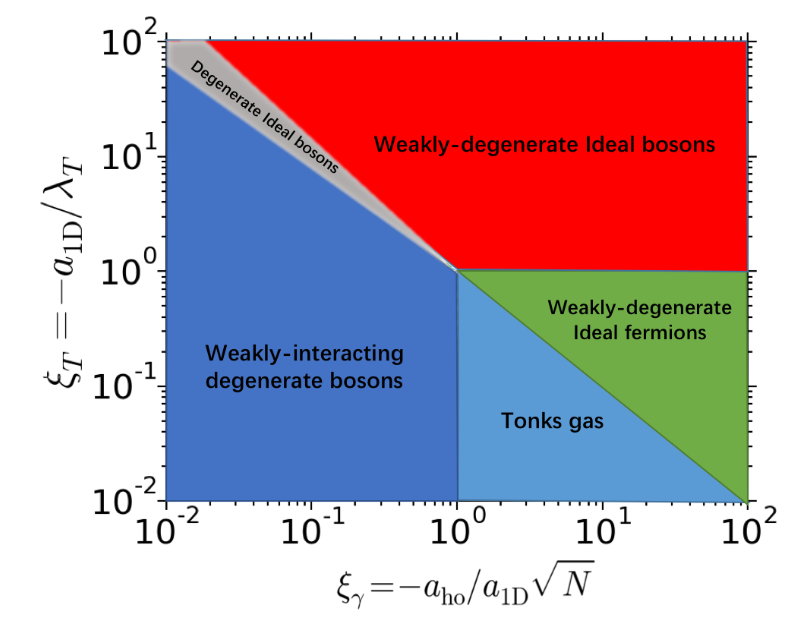
\includegraphics[width=0.8\textwidth]{Fig/Chapter5/state_diagam_hepeng.png}
    \caption[State diagram of trapped 1D Bose gases with repulsive interactions as a function of the reduced temperature $\xi_T$ and the reduced interaction strength $\xi_{\gamma}$ for trapped 1D gases]{State diagram of trapped 1D Bose gases with repulsive interactions as a function of the reduced temperature $\xi_T$ and the reduced interaction strength $\xi_{\gamma}$ for trapped 1D gases. The solid lines indicate smooth crossovers between the different regimes. Taken from \cite{yao:tel-03065015}.}
    \label{fig:1D_diagram}
\end{figure}


\section{Theoretical study}

\label{sec:1D_theory}

Before going into the experimental details, we start our discussion by summarizing the main results of \cite{yao2018tan}. In this theoretical work, the external trapping potential $V$ of equation \ref{eq:lieb_liniger} is taken to be harmonic like in most experiment, including ours. We will write the trapping frequency $\omega_{\rm{1D}}$. 

\subsection{Two-parameter scaling}

At first glance, the physics of the system and in turn Tan's contact should depend from 4 parameters:

\begin{itemize}
    \item The total number of particles $\NBEC$.
    \item The temperature $T$.
    \item The trapping frequency $\omega_{\rm{1D}}$.
    \item The coupling constant $g_{\rm{1D}}$.
\end{itemize}

\noindent The first result of \cite{yao2018tan} is to show that $C$ actually depends from only two parameters, the first one being the reduced interaction strength:

\begin{equation}
    \xi_{\gamma}=-a_{\rm{ho}}/a_{\rm{1D}}\sqrt{N}
    \label{eq:xi_gamma}
\end{equation}

\noindent with $a_{\rm{ho}}=\sqrt{\hbar/m \omega_{\rm{1D}}}$ the harmonic oscillator length and $a_{\rm{1D}}$ the 1D scattering length. The second one is the reduced temperature:

\begin{equation}
    \xi_T=-a_{\rm{1D}}/\lambda_T
\end{equation}

\noindent with $\lambda_T=\sqrt{2\pi \hbar^2/m k_b T}$. The contact can then be written as a function of $\xi_{\gamma}$ and $\xi_{T}$:

\begin{equation}
    C= \frac{N^{5/2}}{a_{\rm{ho}}^3} f(\xi_{\gamma},\xi_{T})
\end{equation}

The goal is then to determine the variations of $f(\xi_{\gamma},\xi_{T})$. To do so, the authors of \cite{yao2018tan} follow two complementary approach. The first one consists in using the Bethe Ansatz which is the exact solution of the Yang-Yang equations \cite{yang1969thermodynamics} of the 1D homogeneous gas. The results are then adapted to the trapped case by using the Local Density Approximation (LDA) in the same fashion of what we did in \ref{sec:ch2_trapping_effects}. The validity of this approach is checked by comparing its prediction to {\it ab-initio} QMC calculations as shown on Fig-\ref{fig:C_theo}.

\begin{figure}
    \centering
    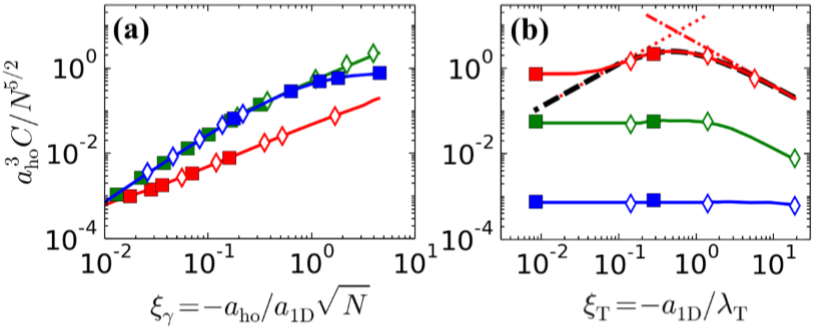
\includegraphics[width=0.9\textwidth]{Fig/Chapter5/BS_LDA_vs_Bethe.PNG}
    \caption[Reduced contact $a_{ho}^3 C / N^{5/2}$ as a function of $\xi_T$ and $\xi_{\gamma}$ as predicted from the LDA approach and QMC calculations]{Reduced contact $a_{ho}^3 C / N^{5/2}$ as a function of $\xi_T$ and $\xi_{\gamma}$ as predicted from the LDA approach (solid lines) and QMC calculations (points). The different symbols correspond to various parameters for the QMC calculations (see \cite{yao2018tan} for further details). (a) Reduced contact versus $\xi_{\gamma}$ at fixed temperatures corresponding to $\xi_T = 0.0085$ (blue), 0.28 (green), and 18.8 (red). (b) Reduced contact versus $\xi_T$  at fixed interaction strengths corresponding to $\xi_\gamma = 10^{-2}$ (blue), $1.58 \times 10^{-1}$ (green), and 4.47 (red). The black dashed, red dotted, and red dash-dotted lines correspond to equations \ref{eq:C_strong_int}, \ref{eq:strong_int_lowT} and \ref{eq:strong_int_highT} respectively.}
    \label{fig:C_theo}
\end{figure}

\subsection{Maximum contact versus temperature}

A striking and unexpected feature of Fig.-\ref{fig:C_theo} panel (b) is that the contact shows a non-monotonous dependency with $\xi_T$ with a maximum, contrary to the monotonous increase in the Tonks-Girardeau regime predicted by \cite{vignolo2013universal}. While the maximum exists for any value of $\xi_{\gamma}$, the effect is more pronounced in the strongly-interacting regime. 

\subsubsection{Strongly-interacting regime}

In this regime, the contact can be determined analytically via a virial expansion \cite{vignolo2013universal} and writes:

\begin{equation}
    C = \frac{2 N^{5/2}}{\pi a_{\rm{ho}}^3} \frac{\xi_\gamma}{\xi_T} \left( \sqrt{2} - \frac{e^{1/2 \pi \xi_T^2}}{\xi_T} \textrm{Erfc}(1/\sqrt{2 \pi} \xi_T) \right)
    \label{eq:C_strong_int}
\end{equation}

In the asymptotic regime of low-temperature limit $\xi_\gamma^{-1} \leq \xi_T \leq 1$, this expression simplifies to:

\begin{equation}
    C = 2 \sqrt{2} \, \frac{N^{5/2}}{a_{ho}^3} \, \xi_\gamma \, \xi_T 
    \label{eq:strong_int_lowT}
\end{equation}

\noindent In the opposite regime of high-temperature $(\xi_\gamma^{-1}, \, 1) \leq \sqrt{\xi_T}$, we rather get:

\begin{equation}
    C \simeq 2 \sqrt{2} \, \frac{N^{5/2}}{ \pi a_{\rm{ho}}^3} \, \frac{\xi_\gamma}{\xi_T} 
    \label{eq:strong_int_highT}
\end{equation}

\noindent We thus clearly see the non-monotonic behavior of the contact with temperature. These 3 expressions are plotted on Fig-\ref{fig:C_theo}. We see that the full analytical expression of \ref{eq:C_strong_int} (black dashed line) well matches the LDA predictions, except for low-temperatures for which the virial expansion is not suited.

The existence of a maximum value of the contact can be understood by the competition between the effect of temperature and interactions. While interaction dominates, the gas is fermionized and the contact increases with temperature \cite{vignolo2013universal}, whereas it decreases as thermal fluctuations take over and fermionization disappears. The location of the maximum of the contact thus provides a way to characterize the crossover to fermionization. 

\subsubsection{Weakly-interacting regime}

In the weakly-interacting regime, the interactions are not strong enough to fermionize the gas. In the low-temperature regime $(1, \, \xi_T) \leq \xi_\gamma^{-1}$, the gas forms a quasi-condensate and the contact is obtained from equation \ref{eq:C_with_int} with the mean-field expression of $\mean{H_{\text {int }}}$ and writes:

\begin{equation}
    C = \eta \frac{N^{5/2}}{a_{\rm{ho}}^3} \xi_\gamma^{5/3} 
    \label{eq:weak_int_lowT}
\end{equation}

\noindent with $\eta = 4 \times 3^{2/3}/5$. We see that $C$ does not depend from temperature here. At high temperatures $\xi_\gamma^{-1} \leq \xi_T \leq \xi_\gamma^{-2}$, interactions become negligible so that the gas is nearly ideal and the contact writes:

\begin{equation}
    C = \left( 16 \sqrt{\pi} \, \frac{N^{5/2}}{a_{ho}^3} \, \xi_\gamma^5 \, \xi_T^3 \right) G(\alpha) \, ,
    \label{eq:weak_int_highT}
\end{equation}

\noindent with $G(\alpha)$ decreasing at least in $\lambda_T^4$ (see \cite{yao2018tan} for the explicit expression), making $C$ decrease with temperature. Once again, identifying the temperature at which $C$ starts to decay allows to characterize the crossover between the quasi-condensate regime and the nearly ideal Bose gas regime.

\section{Experimental realisation of 1D gases with the optical lattice}

\label{sec:1D_exp}

\subsection{2D Lattice}

Now that we have seen what Tan's contact is and how it could be used to characterize the regimes of Lieb-Liniger 1D gases, we show how our experimental apparatus can be adapted to study 1D physics with the objective of testing experimentally the predictions of \cite{yao2018tan}. The main idea to obtain an  experimental 1D system is to ``freeze'' the degrees of freedom of the atoms in two directions of space. To do so, the easiest solution is to use a harmonic trapping potential with trapping frequencies $\omega_{\perp}$ large enough so that the energy difference $\Delta E =\hbar \omega_{\perp}$ between the ground-state and the first excited state is much larger than the typical energy of the atoms $\Delta E \gg \kB T, \mu$ as illustrated on Fig-\ref{fig:1D_config}. Such high trapping frequencies are accessible in our experiment thanks to the optical lattice. Instead of using the 3 pairs of countra-propagating beam as we did so far, we use only 2 such pairs to produce a 2D lattice. Interestingly, the total laser power is divided amongst 2 pair of beams instead of 3, meaning that we can reach much higher values of the lattice depth, typically up to $s=30$. In the direction where there is no lattice, the trapping potential results from the Gaussian shape of the beams and has a trapping frequency $\omega_{\rm{1D}} =2 \pi \times 140 \sqrt{s} = 2 \pi  \times 713 \ \rm{Hz}$ for $s=26$. In the other 2 directions, the trapping frequency is on the contrary very large as a result of the lattice interference pattern $\omega_{\perp} \simeq 200 \ \rm{kHz}$, which is much larger than the energy of the atoms $\kB T, \mu \simeq 25 \ \rm{kHz}$ with typical experimental parameters.

\begin{figure}
    \centering
    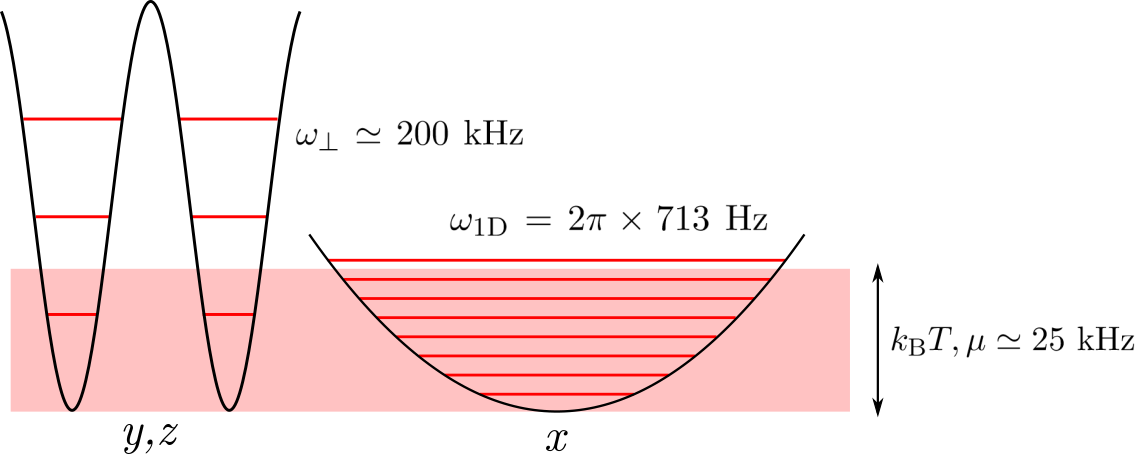
\includegraphics[width=0.9\textwidth]{Fig/Chapter5/1D_config.png}
    \caption[Configuration of the optical lattice to produce 1D tubes]{Configuration of the optical lattice to produce 1D tubes. In the transverse direction, the lattice interference pattern creates a confining potential that can be approximated to a harmonic potential near the center of the site. The trapping frequency is high enough so that the degree of freedom of the atoms in these directions is ``frozen''. On the other hand, the lattice is absent in the longitudinal direction and the trapping frequency only results from the Gaussian shape of the beams. This is the 1D direction.}
    \label{fig:1D_config}
\end{figure}


Using the optical lattice in this configuration then allows us to emulate 1D physics. The main drawback of this method is that we end up with an array of 1D gases rather than a single one, complicating the comparison with theory.


\subsection{Characterization of the 1D tubes}

\subsubsection{Number of atoms}

One major difficulty of working with our array of 1D gases with comes from the fact the atom number varies from one 1D tube to another. To determine the atom number distribution, we first need to determine the density profile of the cloud in the 2D lattice.

To do so, we first remind that under the Thomas-Fermi approximation \cite{pethick2008bose}, the density profile of a BEC in a 3D harmonic potential writes:

\begin{equation}
     n(\bm{r}) = \frac{\mu}{g} \, \left[ 1 - \left( \frac{x}{R_x} \right)^2 - \left( \frac{y}{R_y} \right)^2 - \left( \frac{z}{R_z} \right)^2 \right]
\end{equation}

\noindent where $R_i = \sqrt{\frac{2 \mu}{m \omega_i^2}}$ is the Thomas-Fermi radius in direction $i$ and $g$ the 3D coupling constant already encountered a few times in this manuscript. Under the mean-field approximation, the chemical potential is:

\begin{equation}
     \mu = \frac{\hbar \bar{\omega}}{2} \left(  15 \NBEC \frac{a_s}{a^{\rm{3D}}_{\rm{ho}}}\right)^{2/5}
\end{equation}

\noindent with $\bar{\omega}=\omega_x \omega_y \omega_z/3$ the average trapping frequency with $a^{\rm{3D}}_{\rm{ho}}=\sqrt{\hbar/m \bar{\omega}}$

Similarly to the method developed in \ref{sec:rescaled_interaction}, we rescale the coupling constant $g$ \cite{kramer2002macroscopic} to account for the presence of the 2D lattice:

\begin{equation}
    g'=g\left(\frac{\sqrt{\pi / 2} s^{1 / 4}}{\operatorname{Erf}\left[\pi s^{1 / 4} / 2\right]}\right)^{2}
\end{equation} 

\noindent with the notable difference that we are using here a power 2 instead of power 3 in \ref{sec:rescaled_interaction} as we use here a 2D lattice. We then obtain the rescaled chemical potential:

\begin{equation}
    \mu' = \frac{\hbar \omega_{1D}}{2} \left( 15 N_{tot} \frac{a_s}{a_{\rm{ho}}} g'^2 \right)^{2/5}
\end{equation}

\noindent from which we finally obtain the new Thomas-Fermi radius in the transverse directions:

\begin{equation}
    R_{\rm{TF}} = \frac{1}{d} \sqrt{\frac{2 \mu'}{m \omega_{\perp}^2}}
\end{equation}

\noindent that we express in units of lattice spacing $d$ for convenience. The number of atoms in the tube indexed $j,l$ then writes:

\begin{equation}\label{eq:N_per_tube}
    N_{j,l} = N_{00} \left( 1 - \frac{j^2 + l^2}{R_{\rm{TF}}^2} \right) .
\end{equation}

\noindent where $N_{00}$ is the number of atoms in the central tube. We deduce $N_{00}$ from the total atom number $\NBEC$ with the normalization condition $\NBEC = \sum_{j,l} N_{j,l}$ giving:

\begin{equation}
    N_{00} = \frac{5}{2 \pi} \frac{\NBEC}{R_{\rm{TF}^2}}
\end{equation}

\begin{figure}
    \centering
    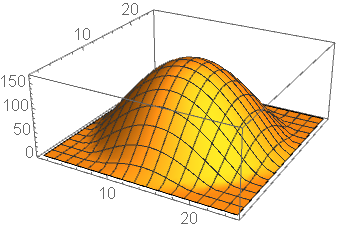
\includegraphics[width=0.6\textwidth]{Fig/Chapter5/atomic_distrib_2Dlatt.PNG}
    \caption{Atom number distribution in a 2D lattice of amplitude $s=26$ for $\NBEC=30 \times 10^3$.}
    \label{fig:my_label}
\end{figure}

\begin{figure}
    \centering
    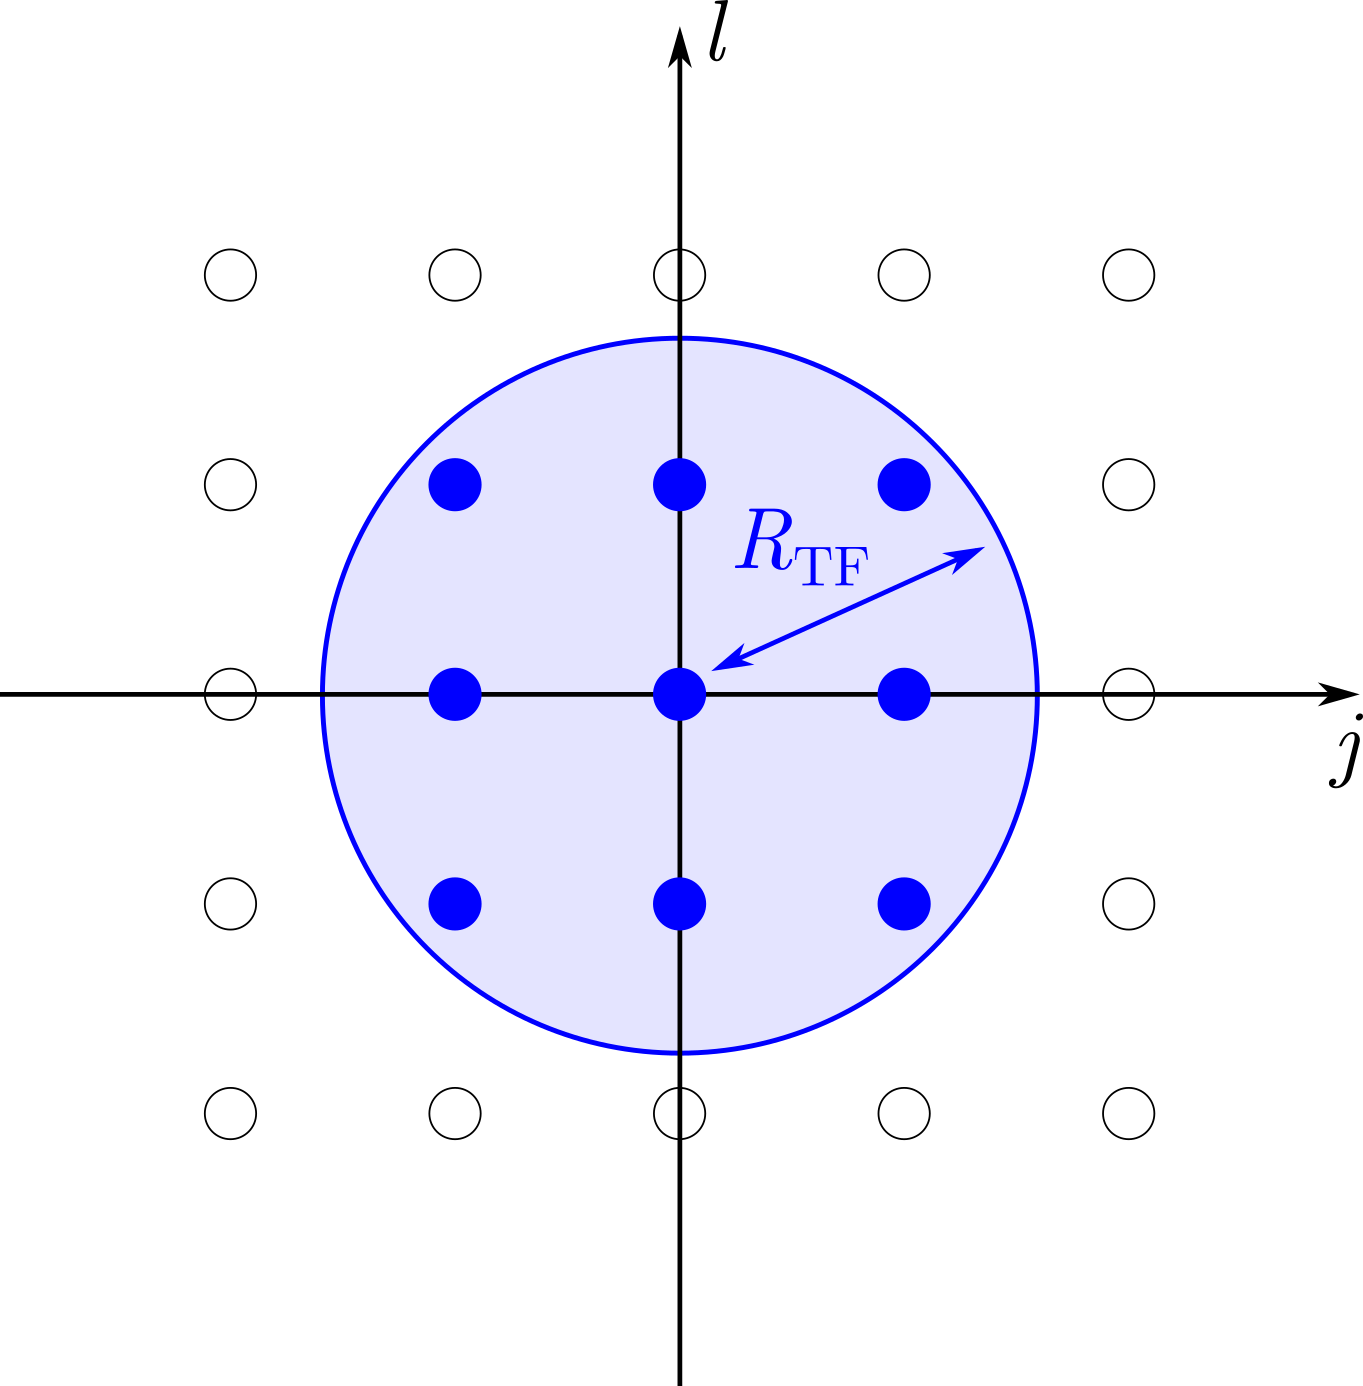
\includegraphics[width=0.45\textwidth]{Fig/Chapter5/tubes_occupes.png}
    \caption[Schematic of the array of 1D tubes]{Schematic of the array of 1D tubes. The large blue circle denotes the parabolic density profile of the BEC that determines which of the lattice sites contain atoms (blue dots).}
    \label{fig:my_label}
\end{figure}

\subsubsection{Density and interaction parameter}


Knowing the number of atom in each tube, it is interesting to determine the density and reduced interaction strength parameter $\xi_{\gamma}$ in each of the tubes. To do so, we first rewrite the 1D interaction strength $g_{\rm{1D}} = 2 \hbar \omega_{\perp} a_s$ \cite{olshanii1998atomic} from the transverse trapping frequency and the 3D scattering length which are our known experimental parameters. We then write the 1D chemical potential and 1D density for the different tubes, both functions of the number of atoms in the tube:

\begin{equation}
    \mu_{1D}^{j,l} = \left( \frac{3}{4 \sqrt{2}} \, N_{j,l}\,  g_{1D} \, \omega_{1D}\,  \sqrt{m} \right)^{2/3}
\end{equation}

\begin{equation}\label{eq:n_1D}
    \rho_{1D}^{j,l}(x) = \frac{\mu_{1D}}{g_{1D}} - \frac{1}{2} \, m \, \omega_{1D}^2 \, x^2
\end{equation}

\noindent In practice, the second term of equation \ref{eq:n_1D} can be neglected because of the small size of the 1D gases $\sim \mu \rm{m}$ and the weak confinement $\omega_{1D} \approx 2 \pi \times 700 \rm{Hz}$ so that $\rho_{1D}^{j,l}(x)$ is constant and well approximated by its value at the center of the trap $\rho_{1D}^{j,l}(0)$. We then simply write $\rho_{1D}^{j,l}$.

% Finally, we can write the interaction parameter $\gamma$ corresponding to the ratio between the interaction and the kinetic energy:

% \begin{equation}
%     \gamma_{j,l} = \frac{m \, g_{1D}}{\hbar n^{j,l}_{1D}} 
% \end{equation}

The reduced interaction strength $\xi_{\gamma}$ is rather straightforward to obtain from the atom number distribution:

\begin{equation}
    \xi_{\gamma}^{j,l}=-a_{\rm{ho}}/a_{\rm{1D}}\sqrt{N_{j,l}}
\end{equation}

\noindent with $a_{\rm{1D}}$ that can be written from the 3D scattering length $a_s$ with $a_{\rm{1D}}=\hbar/m \omega_{\perp} a_s$.

\subsubsection{Weighted average}

\noindent The values of $\xi_{\gamma}^{j,l}$ for each of the 1D tubes are however not very meaningful in practice as the distribution that we measure results from the contribution of every lattice tubes. It is therefore more convenient to define a single averaged value of $\bar{\xi}_{\gamma}$ to approximately describe the entire ensemble of 1D gases. One could first simply think of using a simple average:

\begin{equation}
    \bar{\xi}_{\gamma} = \frac{1}{N_{\rm{tubes}}} \sum_{j,l} \xi_{\gamma}^{j,l}
\end{equation}

\noindent This kind of averaging is however too strong of an approximation as it assumes that each of the tubes contribute equally to the total measured distribution which is wrong as the contribution of the tubes with more atoms will be more significant. We then chose to weight the contribution of each of the tubes in the average by its fraction of the total atom number:

\begin{equation}
    \bar{\xi}_{\gamma} = \sum_{j,l} \frac{N_{j,l}}{\NBEC} \xi_{\gamma}^{j,l}
\end{equation}

\noindent Note that this kind of weighted averaging can be done for all relevant quantities that vary from one 1D tube to another.

\subsubsection{Temperature}

We have proven in \ref{sec:adiabatic_prep} that the loading of the 3D lattice is adiabatic up to lattice depths of $s=18$. As we keep the same loading sequence for the 2D lattice preparing the 1D tubes, it is rather reasonable to assume that the loading is here adiabatic as well even though we go to higher amplitudes and the geometry of the lattice is different. Under this assumption, we then expect the temperature to be the same amongst all the 1D tubes. We will see later how information on the temperature can be obtained from the measured momentum distribution.

\subsubsection{Independence of the tubes}


In order to properly observe 1D physics, it is crucial that all the 1D tubes are independent from one another, \ie no coherence subsists in the transverse directions. This is in principle true when the typical loading time of the lattice set by the slope of the lattice ramps of $0.3 \ \rm{Er}/\rm{ms}$ (see \ref{sec:loading_lattice}) is longer that the decoherence time of the cloud. Practically speaking, we can determine whether the 1D tubes are indeed incoherent or not by looking for diffraction peaks in the transverse directions, as their presence reveals coherent interferences between the different tubes. While we indeed observed no diffraction peaks in most data sets, there were a few occasions where they could be seen, especially for the coldest data sets and lower lattice amplitudes $s \simeq 22$. This calls for a proper study of the decoherence mechanisms happening during the loading of the lattice that has not yet been conducted at the moment where this manuscript is being written. We will for the remainder of this chapter assume that the tubes are indeed independent as the data was taken for relatively high lattice amplitudes $s=26$ at which we observed no diffraction peaks in the transverse direction.

\section{Detection of large momentum components}

\label{sec:large_momentum_detection}

While the great sensitivity of the $\He$ detector is perfectly suited to detect the very low density $\kmf$ momentum tails, its range is inherently limited by the size of the MCPs. This is a major drawback as the $\kmf$ decay only happens for large values of $k$ that might fall out of the range of the $\He$ detector. One solution could be to have the 1D direction vertical as the $\He$ detector range is not limited in this direction, but this is not possible due to the layout of the lattice beams (see \ref{fig:scheme_odt_lattice}). The most advantageous solution is then to set the 1D direction along the direction set by the $+45^{\circ}$ beam (the 2D lattice is then made by the $-45^{\circ}$ and horizontal beams), increasing the effective range of the detector by a factor $\sqrt{2}$. The maximum detectable momentum is then $k_{\rm{max}} \simeq 14 \ \mu \rm{m}^{-1}$.

Actually, we can use the results of \cite{xu2015universal} that show that the $\kmf$ decay should start around $k_0 \sim 1.6 \times \bar{\rho}_{\rm{1D}}$ to determine whether the tails should be detectable or not. For $\NBEC \simeq 100 \times 10^3$, we find that $k_0 \simeq 10 \ \mu \rm{m}^{-1}$, meaning that even though we could see the beginning of the $\kmf$ decay, the range is too small to observe it on a sufficiently large momentum range. We therefore need a solution to effectively increase the momentum range of the $\He$ detector.

\subsection{Magnetic gradient and displacement procedure}

One solution to this issue is to give the entire cloud a momentum kick in the first instants of the TOF to artificially shift the momentum range of the $\He$ detector towards high momenta. With our experimental setup, the easiest way to do so is to create a magnetic gradient to apply a magnetic force on the atoms during a time $t_{\rm{grad}}$ before transferring them to the $m_j=0$ sub-state. 

\subsubsection{New population transfer technique}

This technique however brings some experimental complications as the population transfer cannot be done immediately after turning off the trap. As a matter of fact, the atoms starts moving during the time $t_{\rm{grad}}$ and will therefore be at different positions when the transfer is performed. The problem comes from the fact that there is a slight inhomogeneity in the bias field along direction $x$ used to set the energy difference between the sub-states $m_j=0$ and $m_j=1$, resulting in a small gradient of $0.17 \ \rm{G/cm}$ as already mentioned in \ref{sec:raman}. This means that the resonance condition for a Raman or RF transfer depends on the initial momentum of the atoms, with the consequence that we cannot properly transfer the whole cloud to $m_j=0$ with a simple single frequency Rabi pulse.

To solve this issue, we make use of the Landau-Zener effect that describes the probability for a transition between two levels to occur when the coupling frequency varies linearly in time. As the experiments described in this chapter were performed before the implementation of the two-photon Raman transfer described in Chapter \ref{sec:chapter_3}, this was done by linearly sweeping the frequency $\nu_{\rm{RF}}$ of a RF wave with a span $\Delta \nu_{\rm{RF}}$ around the central resonance frequency $\nu_{\rm{res}} \simeq 12.93 \ \rm{MHz}$ (see \ref{sec:raman}) in a time $\Delta t_{\rm{sweep}}$. The values of $\Delta \nu_{\rm{RF}}$ and $\Delta t_{\rm{sweep}}$ are set according to three constraints.

\begin{itemize}
    \item The initial and final detunings must be much larger than the RF Rabi frequency $\Omega_{\rm{RF}}$ so that $\Delta \nu_{\rm{RF}} \gg 2 \Omega_{\rm{RF}} \simeq 20 \rm{kHz}$
    \item The fraction of transferred atom depends from the rate $\alpha = \Delta \nu_{\rm{RF}}/ \Delta t_{\rm{sweep}}$ at which $\nu_{\rm{RF}}(t)$ changes. The transfer is more efficient as $\alpha$ is low. 
    \item $\Delta \nu_{\rm{RF}}$ must be large enough to encapsulate all resonance frequencies shifted because of the residual magnetic gradient to properly transfer all relevant momentum classes. For an initial momentum $k=-k_d=-8.1 \ \mu \rm{m}^{-1}$, the resonance shift with respect to $k=0$ atoms is around $75 \ \rm{kHz}$ with $t_{\rm{grad}}=13 \ \rm{ms}$.
\end{itemize}

We then decide to set $\Delta \nu_{\rm{RF}}=2 \rm{MHz}$ to make sure that no momentum class is excluded, and set $t_{\rm{sweep}}=3 \ \rm{ms}$ so that $\alpha/\Omega^2_{\rm{RF}}=6.7$, yielding a total detection efficiency $\eta_{\rm{sweep}}=0.10(1)$. We remind that this number accounts for the transfer efficiency which is limited to $50 \%$ because of the three level structure of $2 ^3 S_1$ and the efficiency of the detector itself.

\subsubsection{Generation of the magnetic gradient}

The procedure to create the magnetic gradient was mainly designed to fit the constraints set by the design of our experimental apparatus. As a matter of fact, the geometry of the science chamber makes it quite hard to install coils capable of producing a strong enough gradient along the direction of the $+45^{\circ}$ or $-45^{\circ}$ beams which are the best choice for the 1D direction in terms of momentum range of the detector. On the other hand, there is a gradient coil quite close to the atoms capable of producing a strong enough gradient along the horizontal beam direction that we will denote as the $x$ direction, as well as the MOT coils capable of producing a strong gradient 4 times stronger along $x$. We then decided to set the 1D direction along $x$. While this reduces the momentum range by a factor $\sqrt{2}$, this is not a big issue as we will use the gradient to compensate for it. 

After quite a bit of testing, we decided to use the the MOT coils instead of the $x$ gradient coils as the former is capable of producing a stronger gradient, effectively reducing the time during which the gradient must be applied. This has the advantage of reducing the spatial spread of the atoms before the transfer to $m_j=0$ and thus the inhomogeneity in resonance frequencies because of the residual gradient.  

\subsubsection{Displacement procedure}

The procedure is represented on Fig.-\ref{fig:displacement_sequence}. Right after the lattice is turned off, we increase the current in the MOT coils to produce the magnetic gradient. However, the current in the MOT coils typically needs around $10 \ \rm{ms}$ to reach the highest possible values, which is already quite long. We then set the command voltage $V_{\rm{c}}$ to be close to the highest possible value, let the current increase for $t_1 = 1 \ \rm{ms}$ and then set the command to $0$ and let the current decay for $t_2-t_1=13 \ \rm{ms}$ until it is fully turned off. After that, we finally perform the population transfer and let the atoms fall unto the MCP. The momentum displacement of the cloud can be set by changing the command voltage $V_{\rm{c}}$.

\begin{figure}
    \centering
    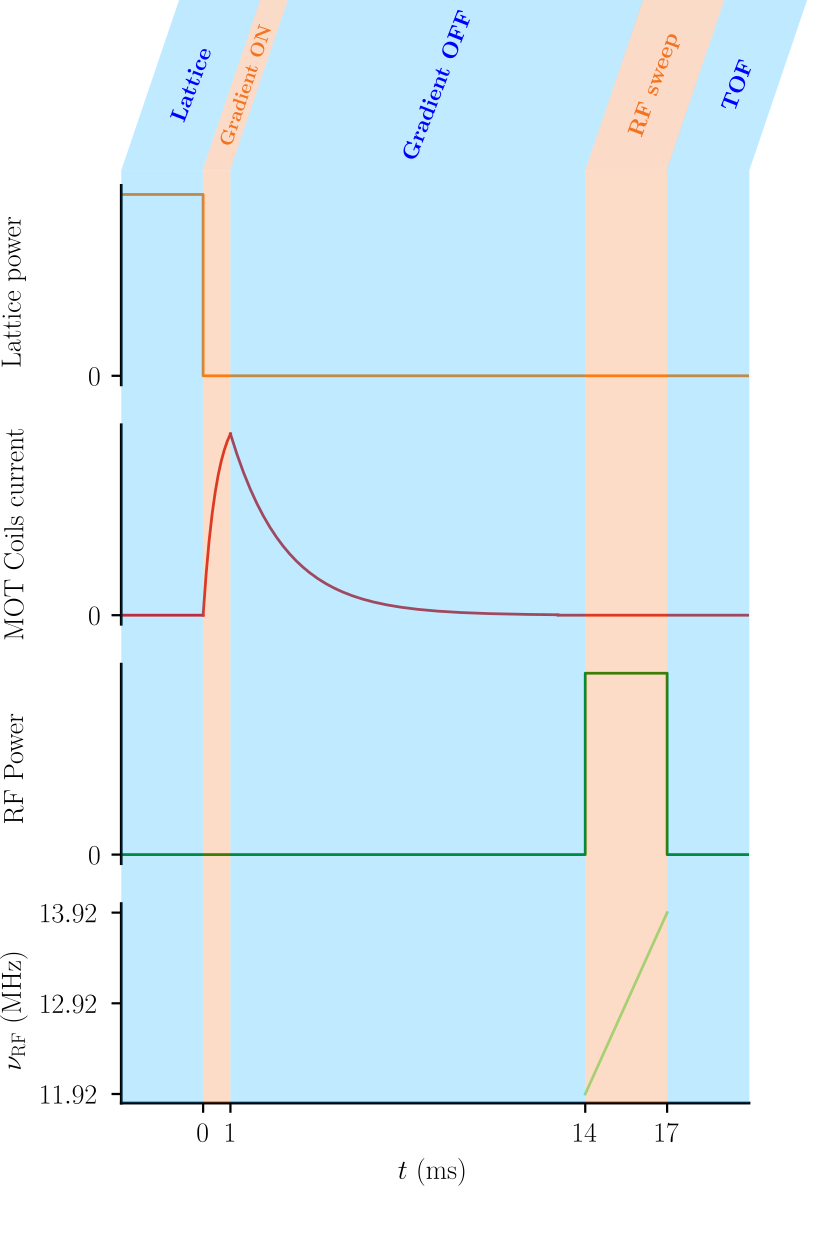
\includegraphics[width=0.8\textwidth]{Fig/Chapter5/displacement_sequence.png}
    \caption[Experimental sequence to shift the entire momentum distribution so that the $\kmf$ tails fall unto the $\He$ detector]{Experimental sequence to shift the entire momentum distribution so that the $\kmf$ tails fall unto the $\He$ detector. The lattice power is represented in orange, the MOT coils current in red and the RF wave power and frequency in green and light green respectively.}
    \label{fig:displacement_sequence}
\end{figure}

\subsubsection{Calculation of the induced displacement}

The effect of the magnetic gradient on the TOF trajectories of the atoms can be calculated rather easily. For simplicity sake, we will assume that the gradient is constant in time and write $B'$ its value along the $x$ axis. The atoms feel a force $F_x=2 \mu_B B'$ for the time $t_{\rm{grad}}$ during which the gradient is on, with $\mu_B$ the Bohr magneton and the factor 2 being the Landé factor. Taking $t=0$ when we start turning on the gradient, the speed of atoms with a zero initial velocity at the center of the trap after $t_{\rm{grad}}$ writes:

\begin{equation}
    v_x(t_{\rm{grad}}) = \frac{2 \mu_B B'}{m} t_{\rm{grad}}
\end{equation}

\noindent In turn, their position writes:

\begin{equation}
    x(t_{\rm{grad}}) = \frac{\mu_B B'}{m} t_{\rm{grad}}^2
\end{equation}

\noindent The final position after the full TOF is linked to $x(t_{\rm{grad}})$ by

\begin{equation}
    x(t_{\rm{TOF}})-x(t_{\rm{grad}}) = v_x(t_{\rm{grad}}) (t_{\rm{TOF}}- t_{\rm{grad}})
\end{equation}

The calculations can be simplified by considering that (1) $t_{\rm{grad}} = 13 \ \rm{ms} \ll t_{\rm{TOF}} = 296 \ \rm{ms}$ and consequently (2) $x(t_{\rm{grad}}) \ll x(t_{\rm{TOF}})$. As a result, the position at the end of the TOF is simply

\begin{equation}
    x(t_{\rm{TOF}})= \frac{2 \mu_B B'}{m} t_{\rm{grad}} t_{\rm{TOF}}
\end{equation}

The effect of the gradient is then simply to shift the position of the entire cloud at the end of the TOF without distorting it, with a simple linear relation between the intensity of the gradient and the value of the position shift.

\subsection{Transverse integration effects and range limitations}

As in \ref{sec:transverse_integration}, the transverse size of the voxels that we will use to compute the momentum density (see \ref{sec:1D_calculation_momentum_density}) defines a transverse integration $\Delta k_{\perp}$ that needs to be sufficiently large $\simeq 0.8 \ \mu \rm{m^{-1}}$ to ensure a proper signal to noise ratio. As illustrated on Fig.\ref{fig:1D_integration}, the transverse integration however effectively reduces the momentum range in the 1D direction because of the circular shape of the detector that cuts out a part of the integration volume. The transverse integration must then be kept as low as possible and the distorted edges of the distribution ignored in the analysis. 

\begin{figure}
    \centering
    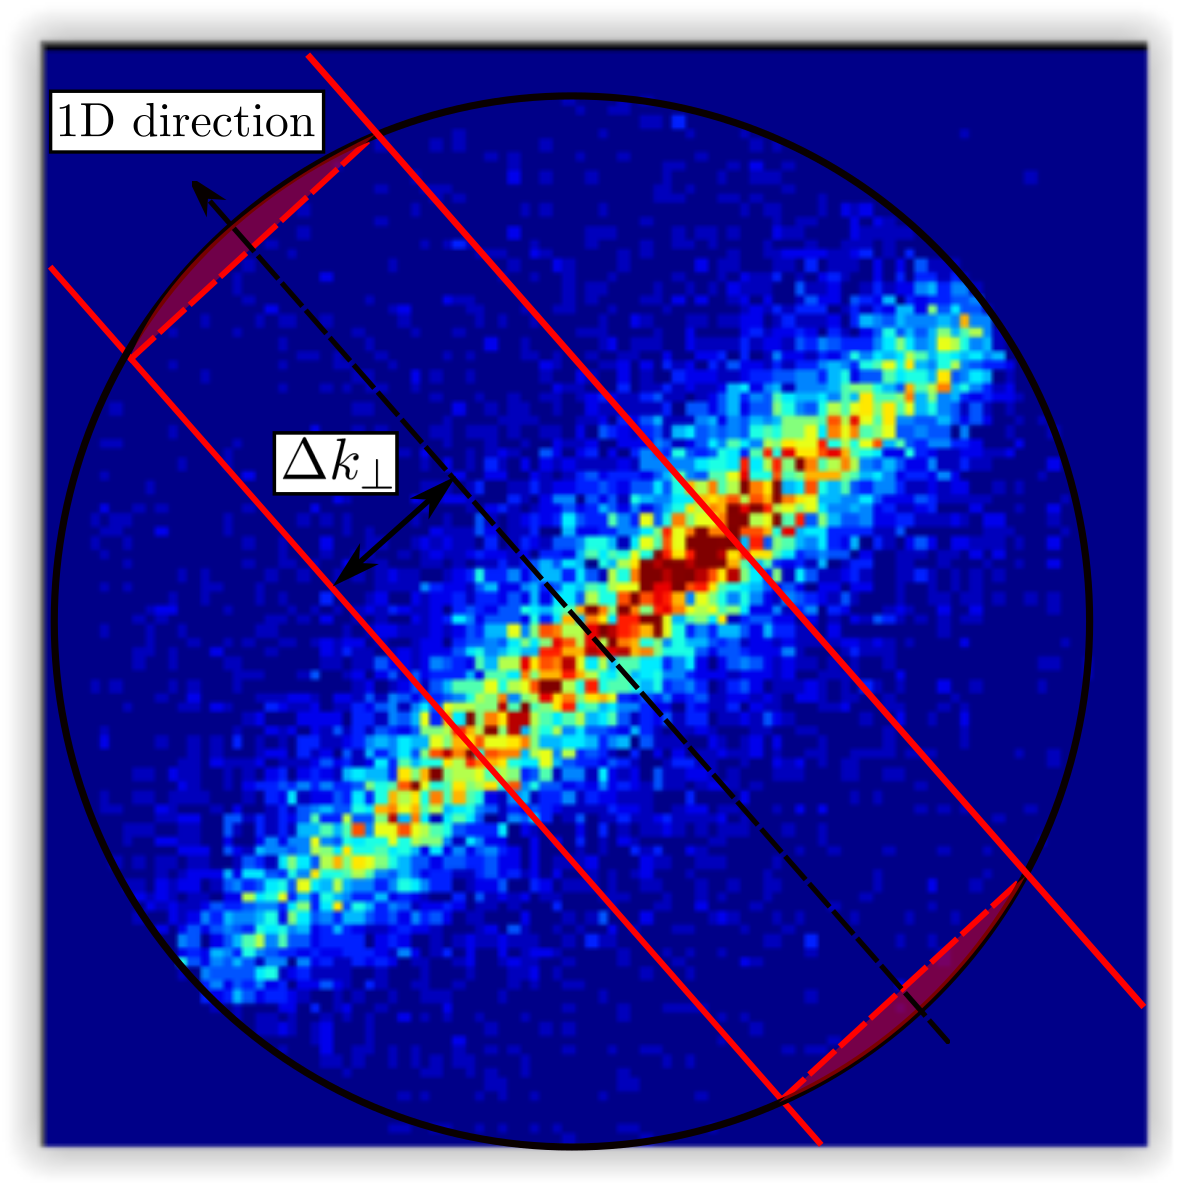
\includegraphics[width=0.7\textwidth]{Fig/Chapter5/1D_transverse_integration.png}
    \caption[Effect of the transverse integration of 1D gases data]{Gravity integrated 2D image of the distribution of the 1D lattice gas illustrating the effect of the transverse integration. The red shaded area indicated the region where the geometry of the detector affects the measurement of $n_{\rm{1D}} (k)$.}
    \label{fig:1D_integration}
\end{figure}

\subsection{Benchmarking with 3D lattice gases momentum distribution}

To check that our method does not induce any distortion of the momentum distribution, we benchmark it with 3D lattice gas momentum distribution for different displacements. The lattice amplitude is set to $s=15$, \ie high enough so that the momentum distribution has a wide background but still sharp diffraction peaks. We can check the overlap of the data sets for different displacements with the wide background while precisely characterizing distortion effects by looking at the location of the diffraction peaks.

\begin{figure}
    \centering
    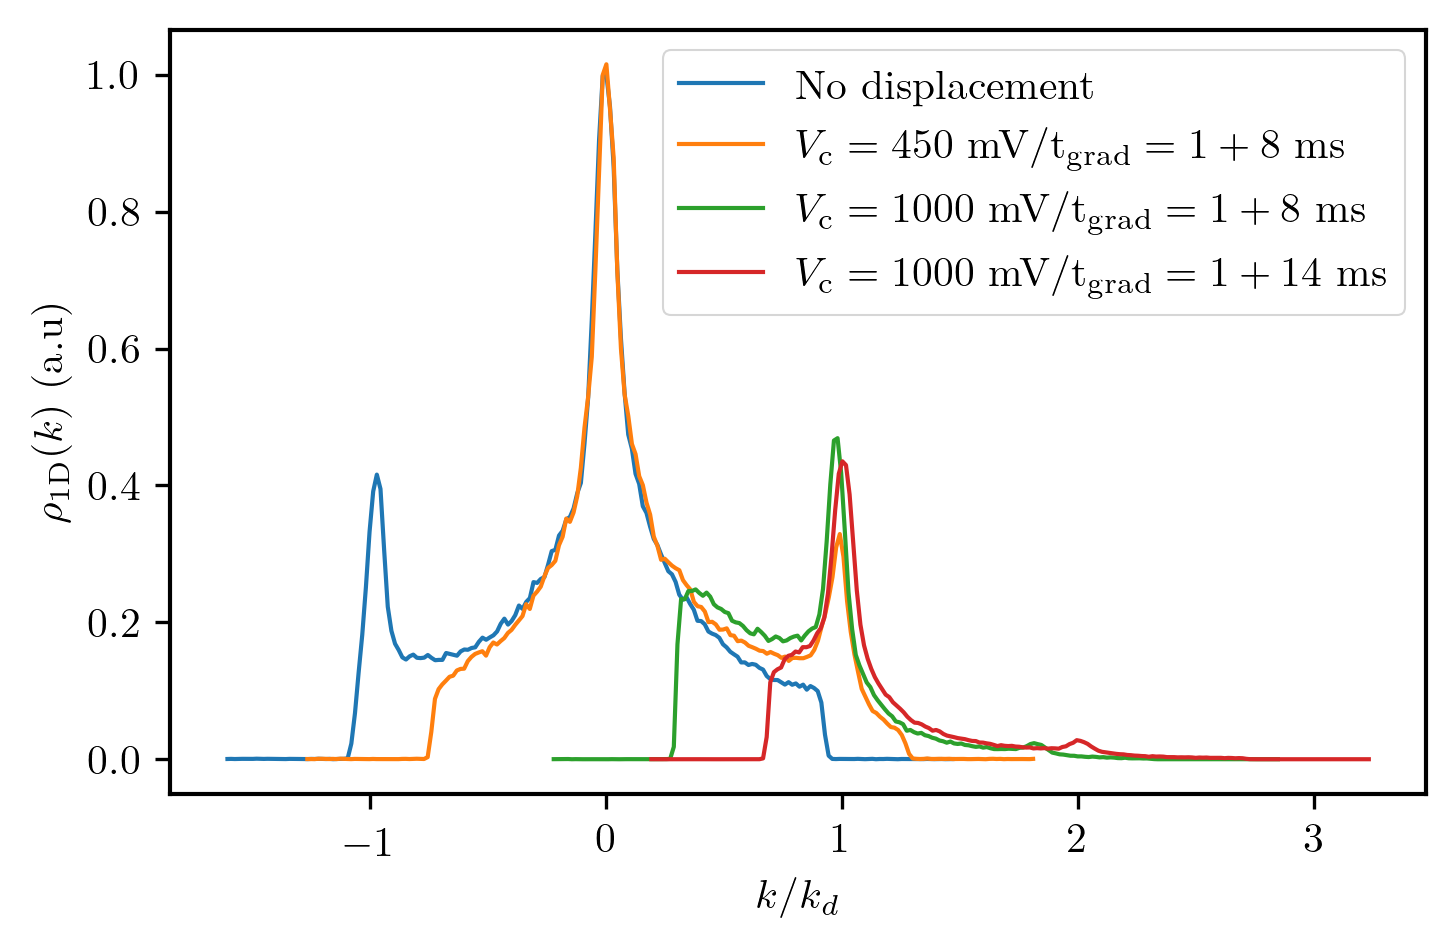
\includegraphics[width=0.9\textwidth]{Fig/Chapter5/overlap.png}
    \caption[Test of the displacement sequence on a 3D lattice $s=15$ momentum distribution]{Test of the displacement sequence on a 3D lattice $s=15$ momentum distribution. The blue curve corresponds to no displacement gradient, while the orange, and green curves corresponds to displaced data with a command voltage $V_{\rm{c}}=450 \ \rm{mV}$ for the orange curve and $V_{\rm{c}}=1000 \ \rm{mV}$ for the green one. The time $t_{\rm{grad}}$ before the RF transfer consists $1 \ \rm{ms}$ during which the current in the MOT coils is set to increase, and $8 \ \rm{ms}$ where it is left to decrease for the orange curve. This time is extended to $14 \ \rm{ms}$ for the green curve.}
    \label{fig:1D_overlap_mott}
\end{figure}

\begin{figure}
    \centering
    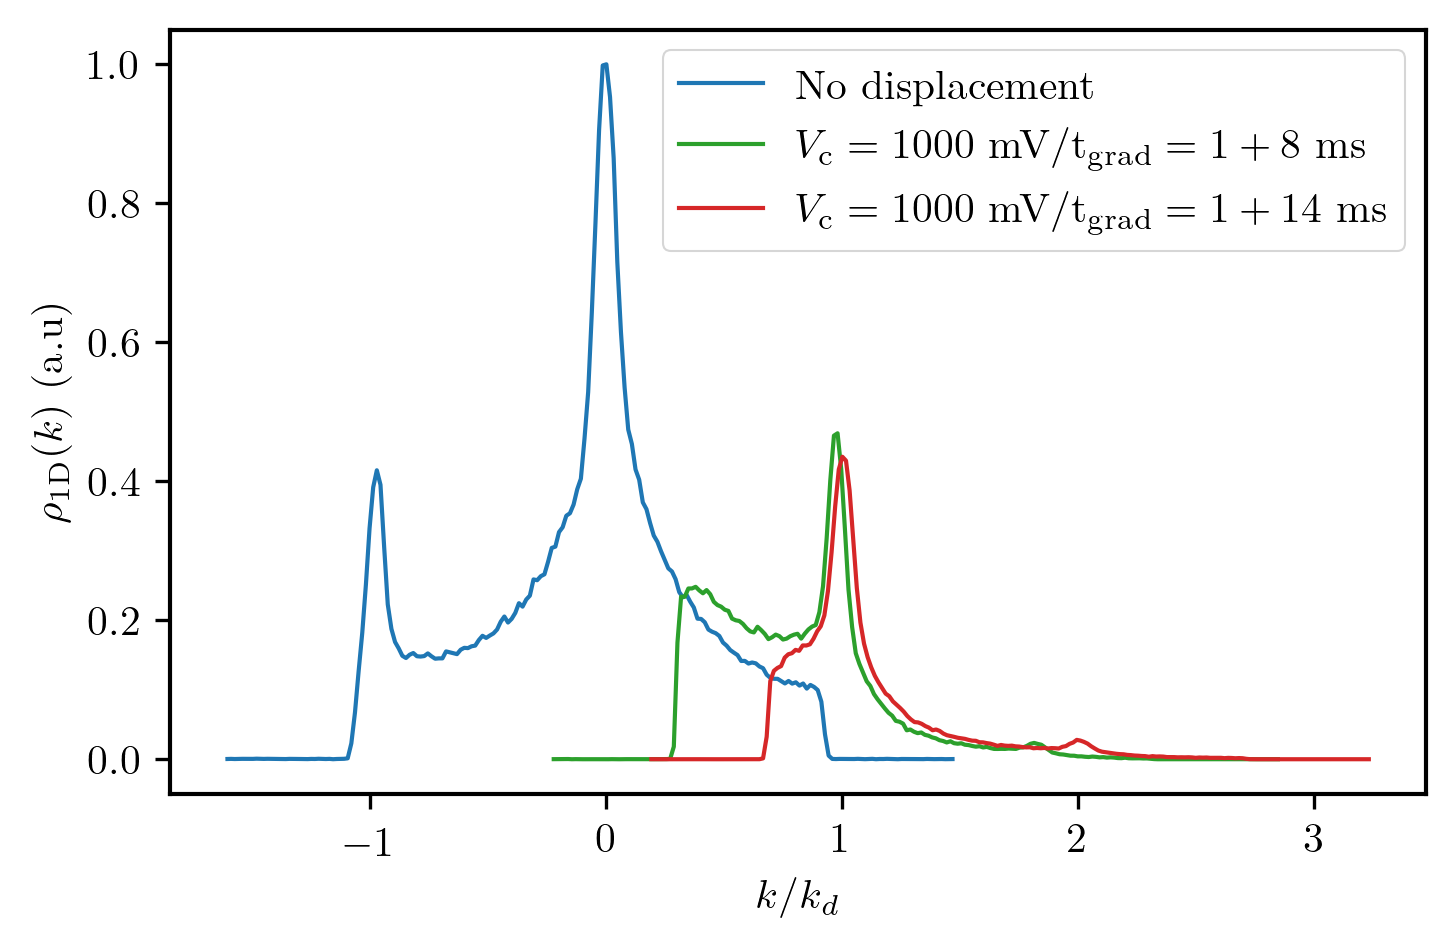
\includegraphics[width=0.9\textwidth]{Fig/Chapter5/bad_overlap.png}
    \caption[Distortion of the momentum distribution]{Distortion of the distribution. The parameters are the same than for Fig.-\ref{fig:1D_overlap_mott} with the addition of the red curve corresponding to a command voltage $V_{\rm{c}}=1000 \ \rm{mV}$ and $t_{\rm{grad}}$ of $1 \ \rm{ms}$ during which the current in the MOT coils is set to increase and $8 \ \rm{ms}$ where it is left to decrease. As this time is too small for the strong gradient too be properly turned off, the distribution is distorted explaining why the diffraction peak appears at lower $k$ value.}
    \label{fig:1D_bad_overlap_mott}
\end{figure}



The data is plotted on Fig-\ref{fig:1D_overlap_mott} and Fig-\ref{fig:1D_bad_overlap_mott}. These two figures illustrate several crucial points:

\begin{itemize}
    \item Even though we get an almost perfect agreement between the blue (non-displaced) and the orange curve on Fig.-\ref{fig:1D_overlap_mott}, the orange peak at $k=k_d$ is lower than expected. This is an effect that we attribute to the transverse integration that causes the measured distribution to decay faster than we would expect on the edges of the MCP as explained in the previous paragraph. The green curve however well reproduces the shape of the $-1 \ k_d$ peak. 
    
    \item The red curve of Fig-\ref{fig:1D_bad_overlap_mott} illustrates an important caveat of the displacement procedure. While we still let the current in the MOT coils increase for $1 \ \rm{ms}$, we perform the RF transfer only $8 \ \rm{ms}$ after this step which is too short for the gradient to properly turn off, contrary to the green curve where this time is increased to $14 \ \rm{ms}$. Because of the distance travelled by the atoms before the RF sweep and the presence of a gradient, the atoms see different magnetic fields and thus have different resonance frequencies depending on their initial momentum. When the RF sweep is performed, some atoms will then be transferred later than others and will thus interact longer with the magnetic field, resulting in a larger displacement and a distortion of the distribution. This effect is striking on the red curve for which the diffraction peak appears at a lower $k$ than expected. On the other hand, if we wait long enough for the displacement gradient to be turned off, this effect disappear as illustrated by the diffraction peak of the green curve well centered on $k=k_d$.
\end{itemize}

Overall, we get a nice overlap between the different properly displaced data sets and therefore conclude that our displacement method does not induce any distortion of the measured momentum distribution. 

\section{Experimental study}

Having described the experimental procedure to collect the data, we detail in this section the techniques and crucial points to properly analyze the experimental data.

\subsection{Analysis of the transverse shape}

The first point that we need to check is the transverse shape of the 3D distribution to know whether we can fully decouple what is happening in the 1D direction from what is happening in the other two transverse directions. The transverse momentum distribution is supposed to be a Gaussian distribution whose width depends on the transverse trapping frequency. If the atoms are in the harmonic oscillator ground state of the transverse direction, the RMS width of the distribution in momentum-space is $\sigma_{\rm{theo}}=\sqrt{\frac{m \omega_{\perp}}{2 \hbar}}$. 

On Fig.-\ref{fig:1D_transverse}, we plot the transverse distribution along gravity at different positions along the 1D direction and normalize it to 1. We observe that we get the same RMS size for every $k_{\rm{1D}}$ at which the cut is done meaning that the 1D direction is fully decoupled from what is happening in the transverse direction. We extract its RMS width \fcolorbox{red}{white}{$\sigma_{\rm{exp}}=5.96(2) \mu \rm{m}^{-1}$}. This data set was taken with $s=26$, meaning that $\omega_{\perp}= 1.33(3) \times 10^6 \ \rm{s}^{-1}$ (see \ref{label:formule_wL} for the detailled formula), giving \fcolorbox{red}{white}{$\sigma_{\rm{theo}}=6.4(1) \ \mu \rm{m}^{-1}$} so a slight discrepancy. This could be explained by the fact that a few atoms (a few percents of the total atom number) are in the first excited state with a larger spatial extent and thus and smaller momentum width.

\begin{figure}
    \centering
    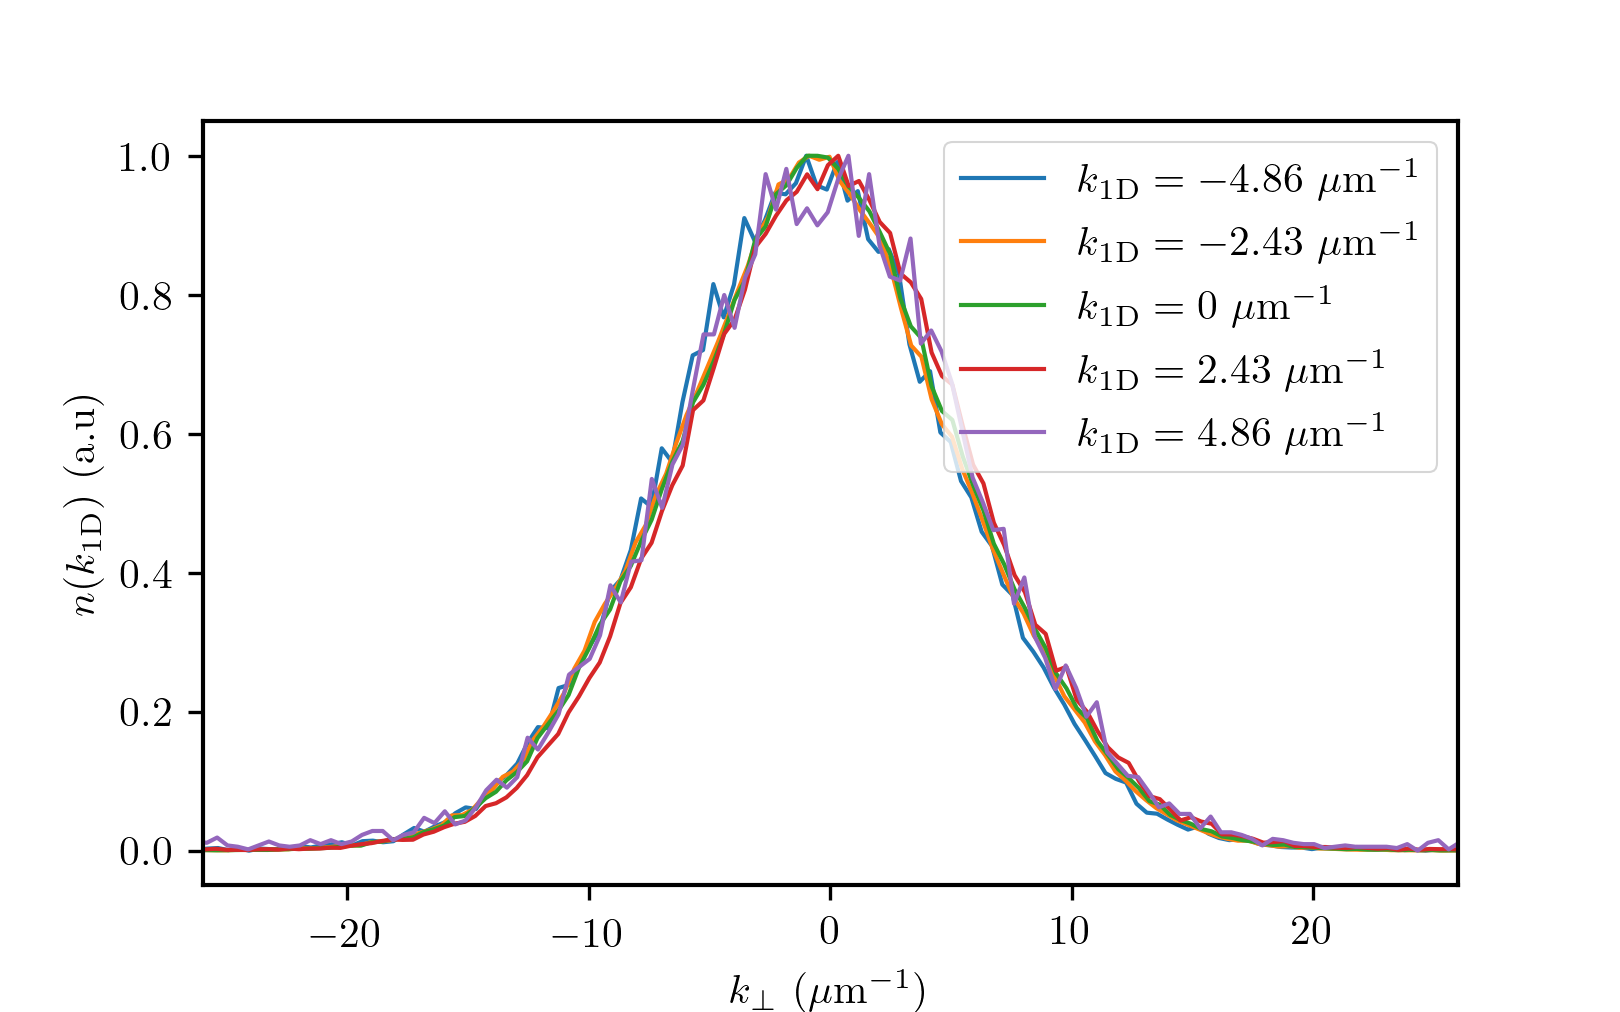
\includegraphics[width=0.9\textwidth]{Fig/Chapter5/1D_transverse_effect.png}
    \caption[Normalized 1D cut along gravity of the experimental distribution at various $k$ along the 1D direction]{Normalized 1D cut along gravity of the experimental distribution at various $k$ along the 1D direction. The Gaussian shape remains unchanged, meaning that the 1D direction is fully decoupled from the transverse directions.}
    \label{fig:1D_transverse}
\end{figure}

\subsection{Calculation of the momentum density}


\label{sec:1D_calculation_momentum_density}

In order to compare the experimental values of the Tan's contact to theory, it is crucial to obtain the absolute value of the 1D density $\rho_{\rm{1D}}(k)$ from the experimental data. To do so, we exploit the fact that the transverse distribution shape is the same along the 1D direction as we have just seen. Under the effect of the fast transverse expansion, some atoms fall beyond the MCP and are therefore not detected. However, knowing the transverse profile, we can do as if everything was only happening in one direction and integrate over the transverse profile. The procedure is the following:

\begin{itemize}
    \item We plot the transverse distribution (in the vertical direction where it is not cut out by the finite size of the $\He$ detector) and extract its RMS width $\sigma_{\rm{exp}}$.
    \item For one voxel of size $\Delta k_{1D} \times \Delta k_{\perp}^2$, we have (keeping in mind normalization condition with the factor $2\pi$):
    

    \begin{align}
        \rho_{1D}(k) &= 2\pi \times \frac{N_{\rm{vox}}(k)}{\eta_{\rm{sweep}} \Delta k_{1D} \Delta k_{\perp}^2} \left(\int \rho_{\perp}(k) dk \right)^2 \\
        % &=2\pi \times \frac{N_{\rm{pix}}(k)}{\eta \delta k_{1D} \delta k_{\perp}^2} 2 \pi \sigma 
    \end{align}
    
    \noindent $\eta_{\rm{sweep}}$ being the detection efficiency and $N_{\rm{vox}}$ the number of atoms in the voxel at a given $k$. From this, we obtain the expression of $\rho_{\rm{1D}}(k)$ that depends only on measured experimental values:
    
    \begin{equation}
        \rho_{1D}(k) = 4\pi^2 \times \frac{N_{\rm{vox}}(k)}{\eta_{\rm{sweep}} \Delta k_{1D} \Delta k_{\perp}^2} \sigma_{\rm{exp}^2} 
    \end{equation}

    

\end{itemize}



\subsection{Measurement of the temperature}

\label{sec:1D_temperature}

As we want to study the dependency of the Tan's contact with temperature and compare with {\it ab-initio} QMC calculations, we first need to extract the temperature from the experimental data. Actually, the width of the momentum distribution contains information about the temperature under certain conditions that we will now discuss.

We need to look at the properties of the first order spatial correlation function which is directly reflected in the momentum distribution. In 1D gases at $T=0$, the interactions induce an algebraic decay of the first order correlation function that translates into an algebraic decay of the momentum distribution \cite{gangardt2003stability,pitaevskii1991}. However, at $T \neq 0$, the temperature creates phase fluctuations that induce an exponential decay of the first order correlation function. In the weakly-interacting regime where $(1, \, \xi_T) \leq \xi_\gamma^{-1}$, this decay happens on shorter length scales than the one induced by interactions. This means that at low $k$, the momentum distribution is Lorentzian (Fourier transform of a damped exponential) \cite{cazalilla2004bosonizing,fabbri2011momentum,gerbier2004condensat}:

\begin{equation}
    \rho_{\rm{1D}}(k)=\frac{2 \bar{\rho}_{\rm{1D}}(0)/\delta k }{1+(k/\delta k)^2}
\end{equation}

\noindent with $\bar{\rho}_{\rm{1D}}(0)$ the average central density over the tubes weighted by the number
of atoms in the tube. Its width $\delta k$ is linked to the coherence length of the gas $L_{\rm{\phi}}$:

\begin{equation}
    \delta k= \frac{\alpha_{\rm{fit}}}{L_{\phi}} 
\end{equation}

\noindent itself linked to temperature by:

\begin{equation}
    {L_{\phi}} = \frac{\hbar^2 \bar{\rho}_{\rm{1D}}(0)}{m \kB T}
\end{equation}

\noindent where $\alpha_{\rm{fit}}$ is a coefficient that depends from the 1D trapping frequency $\omega_{\rm{1D}}$ and the interaction parameter. It is not entirely clear whether this picture should hold for our typical experimental parameters putting us near the frontier between the the weakly-interacting and strongly interacting regimes. However, numerical QMC calculations performed by Hepeng Yao from Centre de Physique Théorique at Ecole Polytechnique have shown that this description works, provided that the proper $\alpha_{\rm{fit}}$ is used. Its value has been calibrated with the QMC calculations and is typically equal to $\alpha_{\rm{fit}} = [0.78,0.79]$ for the data sets presented here. The temperature of the system can then easily be extracted with a Lorentzian fit of the measured momentum distribution at low $k$ as illustrated on Fig-\ref{fig:1D_temperature}.

\begin{figure}
    \centering
    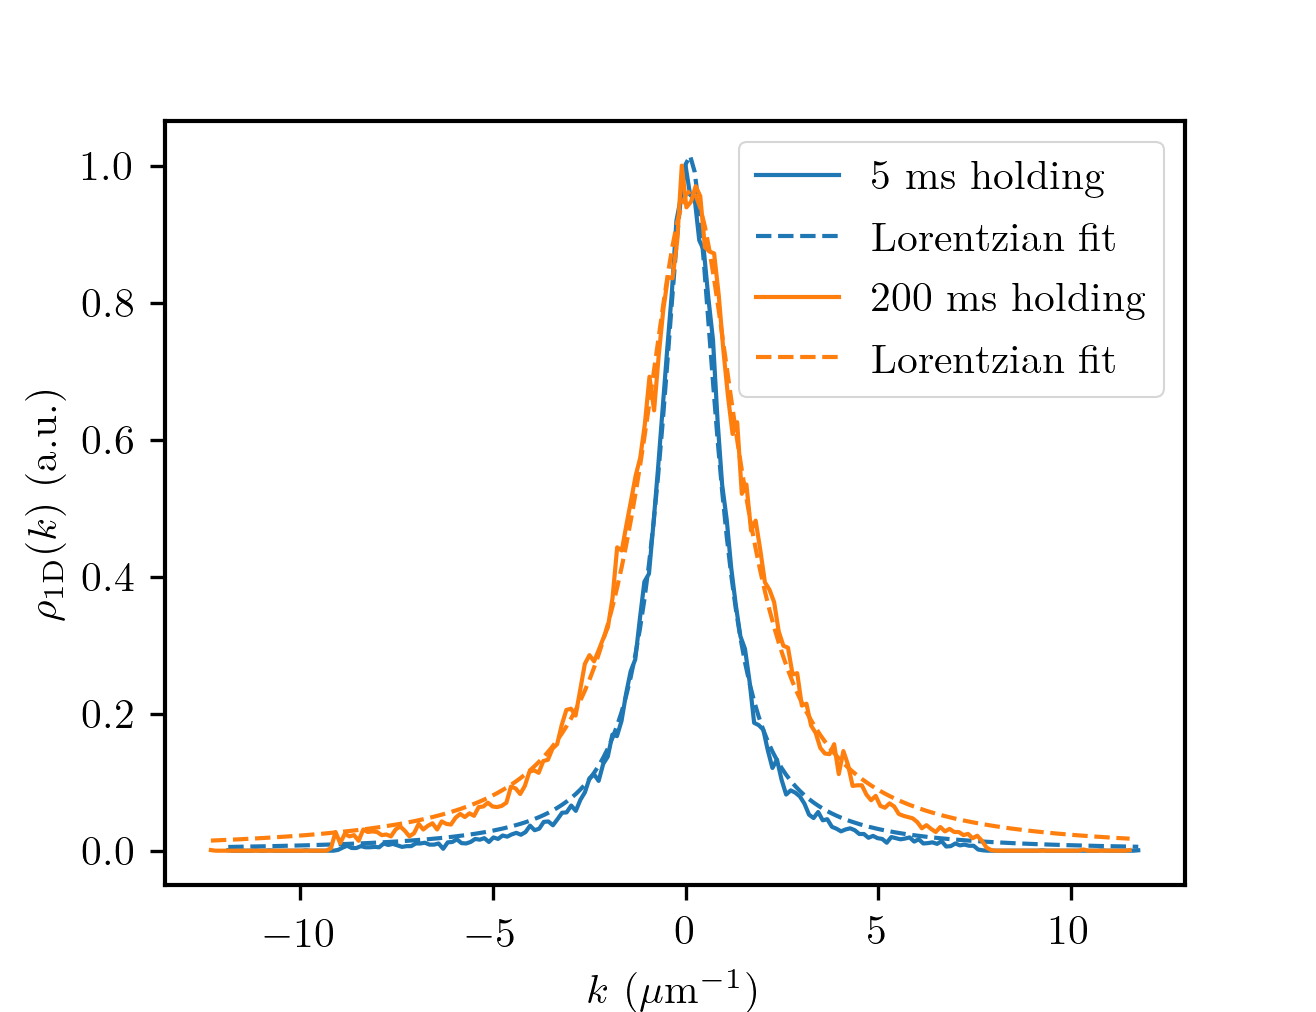
\includegraphics[width=0.8\textwidth]{Fig/Chapter5/1D_temperature_lorentz.png}
    \caption[Normalized 1D momentum distribution $\rho_{\rm{1D}} (k)$ for lattice holding times $t_{\rm{hold}}=5 \ \rm{ms}$ and $t_{\rm{hold}}=200 \ \rm{ms}$]{Normalized 1D momentum distribution $\rho_{\rm{1D}} (k)$ for lattice holding times $t_{\rm{hold}}=5 \ \rm{ms}$ and $t_{\rm{hold}}=200 \ \rm{ms}$. The Lorentzian fit well matches the data at low $k$. The increase in the width of the distribution signals the increase in temperature induced by the increased holding time in the lattice. We measure $T=800 \ \rm{nK}$ for $t_{\rm{hold}}=5 \ \rm{ms}$ and $T=1.5 \ \mu \rm{K}$ for $t_{\rm{hold}}=200 \ \rm{ms}$.}
    \label{fig:1D_temperature}
\end{figure}

In practice, the temperature can be increased in the same fashion than described in \ref{sec:kmk_temperature} by increasing the holding time in the lattice. This effect is clearly visible in Fig-\ref{fig:1D_temperature} where we see that the width of the Lorenztian increases when the holding time is increased. Table \ref{tab:T_vs_t_hold} shows the temperatures, lattice holding times and reduced temperatures of the 3 data sets presented in this chapter. 

\begin{table}[h!]
\centering
{\rowcolors{2}{white}{MainColor!12}
    \begin{tabular}{c|c|c}
        {\color{MainColor} $t_{\rm{hold}} \ (\rm{ms})$} &  {\color{MainColor}$T \ (\mu \rm{K})$} & {\color{MainColor}$\xi_T$} \\
        \hline
        5 & 0.8 & 1.57 \\
        200 & 1.5 & 2.09 \\
        600 & 2.9 & 2.91 \\
    \end{tabular}}
\caption{Temperature of the system for 3 lattice holding times $t_{\rm{hold}}$ and corresponding reduced temperature $\xi_T$.}
\label{tab:T_vs_t_hold}
\end{table}


\subsection{Interaction parameter}

The other relevant parameter affecting the value of Tan's contact besides temperature is the reduced interaction strength as defined in equation \ref{eq:xi_gamma} which we control by changing the total number of atoms $\NBEC$ loaded in the 2D optical lattice. Table \ref{tab:gamma_vs_N} shows its weighted average values versus the total atom number $\NBEC$ for the 3 data sets that we will be discussed here.


\begin{table}[h!]
\centering
{\rowcolors{2}{white}{MainColor!12}
    \begin{tabular}{c|c|c}
        {\color{MainColor} $\NBEC$} &  {\color{MainColor}$\bar{N}$} & {\color{MainColor}$\bar{\xi}_{\gamma$} \\
        \hline
        3.1 $\times 10^4$  & 58 & 0.167 \\
        1.1 $\times 10^5$ & 125 & 0.113 \\
        2.3 $\times 10^5$ & 192 & 0.092 \\
    \end{tabular}}
\caption{Weighted average number of atoms per tube and average reduced interaction strength for 3 different total atom numbers $\NBEC$.}
\label{tab:gamma_vs_N}
\end{table}

\subsection{Experimental procedure and first extracted values of the Tan's contact}

The procedure to measure Tan's contact for a given data set is as follows:

\begin{itemize}
    \item We prepare the parameters of the experiment to reach the desired values of temperature and atom number. The latter is calibrated via absorption imaging while the former is set by changing the holding time in the lattice and checking that the width of the 1D distribution increases. 
    \item We start by taking $\sim 100$ experimental shots with no gradient to measure the low $k$ distribution from which we can extract the temperature as explained in \ref{sec:1D_temperature}. We do not need to take a large number of shots as the signal is quite high and we do not require a very high signal to noise ratio to obtain the temperature.
    \item We set the gradient to shift the momentum distribution to access the momentum region where the the $\kmf$ tails are supposed to be present as explained in \ref{sec:large_momentum_detection}. Usually, the displacement is not too high so that the momentum range overlaps the natural momentum range of the $\He$ detector where no gradient is used, allowing to check that the displaced data matches nicely the non displaced data in the region of the overlap as shown on Fig.-\ref{fig:1D_plots} panels (a) and (b). In the following for clarity sake, we will plot one single curve obtained by merging the low and high momentum data.
    \item After computing the 1D distribution $\rho_{\rm{1D}} (k)$ with the method detailed in \ref{sec:1D_calculation_momentum_density}, we plot the quantity $\rho_{\rm{1D}} (k) \times k^4$. The presence of $\kmf$ tails is signaled by a flat zone that we can fit with a constant function to extract the bare value of the contact $C$ as illustrated on Fig.-\ref{fig:1D_plots}.

    
\end{itemize}  
    
\begin{figure}
    \centering
    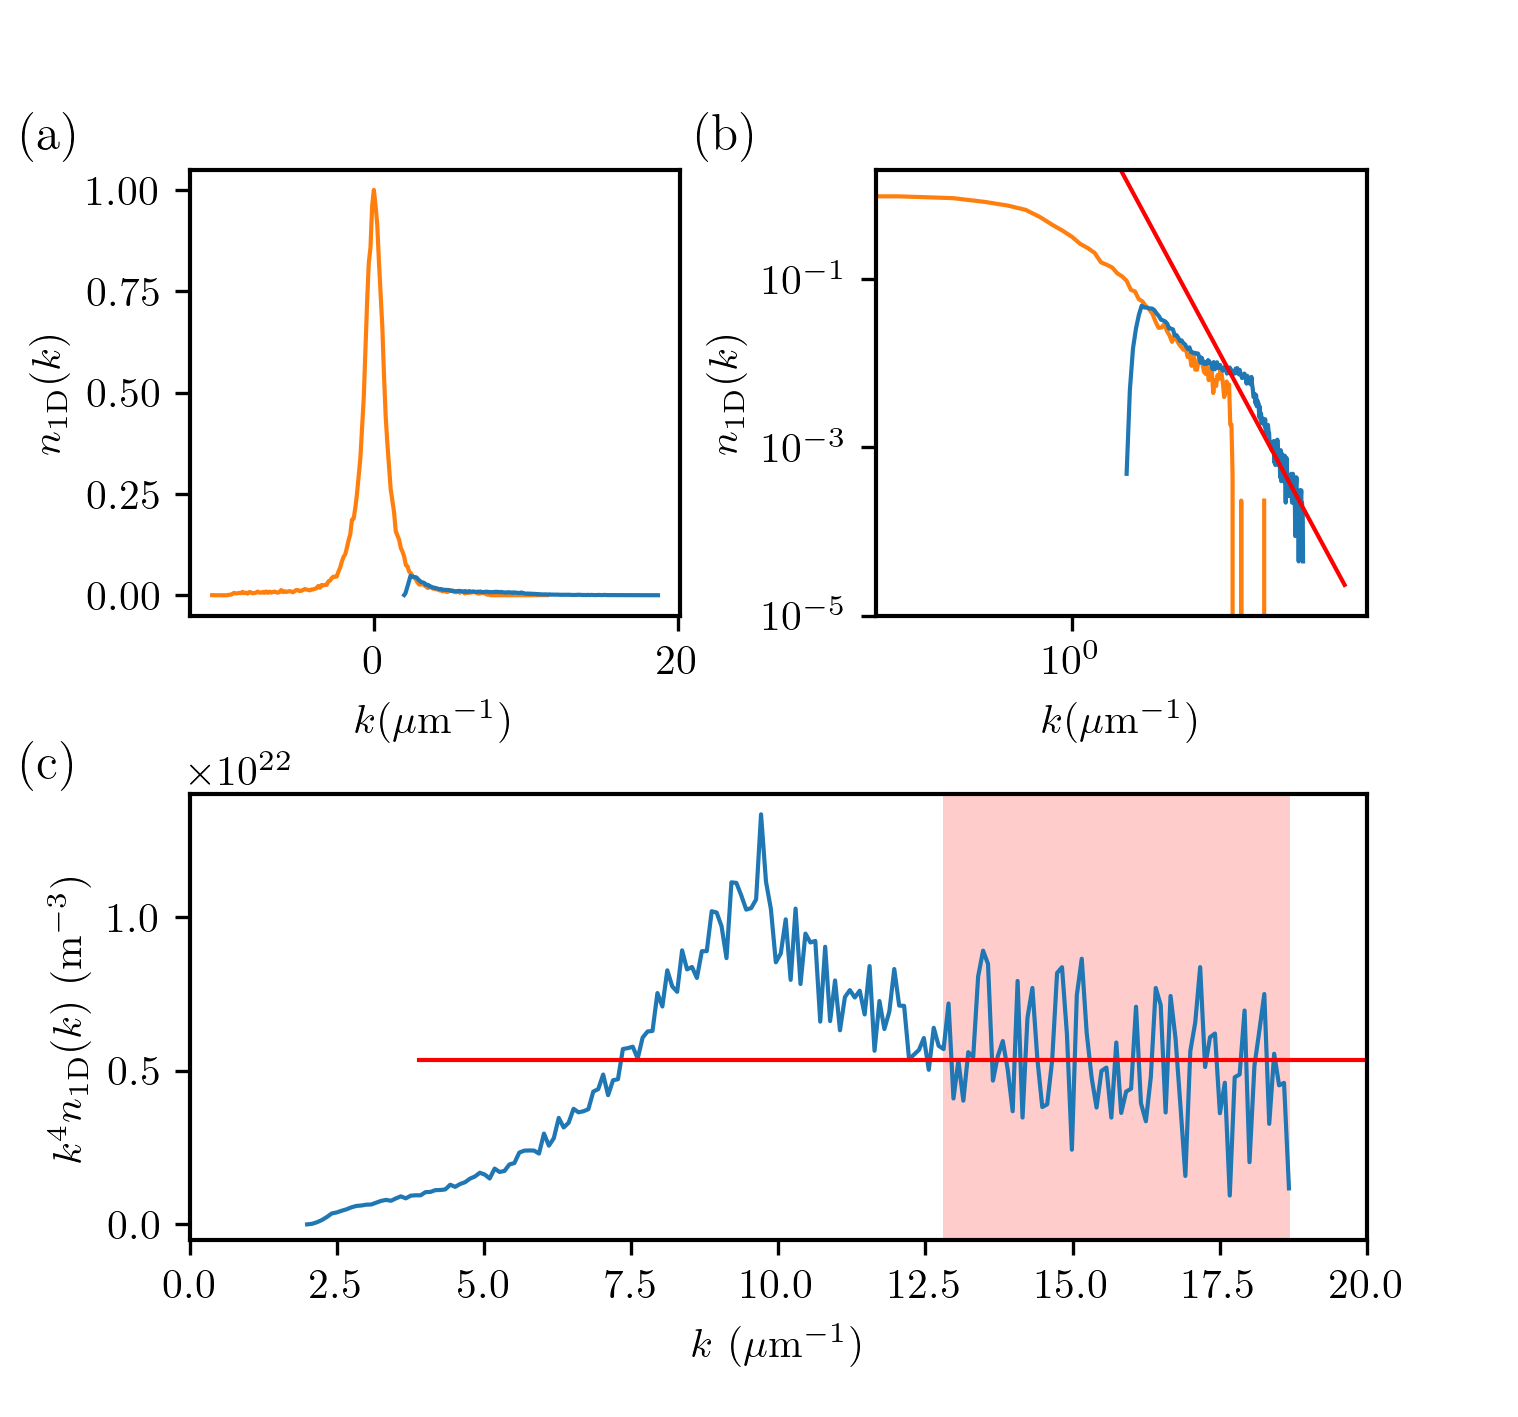
\includegraphics[width=0.95\textwidth]{Fig/Chapter5/1D_plots.png}
    \caption[Plots of $\rho_{\rm{1D}}(k)$ for $s=26$, $N=3.1(3) \times 10^4$ and $t_{\rm{hold}}=5 \ \rm{ms}$]{Plots of $\rho_{\rm{1D}}(k)$ for $s=26$, $N=3.1(3) \times 10^4$ and $t_{\rm{hold}}=5 \ \rm{ms}$. (a) Linear scale plot of the normalized $\rho_{\rm{1D}}(k)$ for two momentum ranges. (b) Same data in log scale. The red line indicates a $k^{-4}$ fit. (c) $k^4 \rho_{\rm{1D}} (k)$ at high momentum. The red shaded area indicates the flat zone of the $\kmf$ tail.}
    \label{fig:1D_plots}
\end{figure}

Coming back to the predictions of \cite{yao2018tan}, we have already seen that the contact can be written:

\begin{equation}
    C= \frac{N^{5/2}}{a_{\rm{ho}}^3} f(\xi_{\gamma},\xi_{T})
\end{equation}

\noindent We can then define a rescaled contact:

\begin{equation}
    \tilde{C}=C \frac{a_{\rm{ho}}^3}{N^{5/2}}
\end{equation}

\noindent as plotted on Fig-\ref{fig:C_theo}. In the following, we will then plot $\tilde{C}$ instead of the bare value $C$ for convenience.


\section{Discussion of the preliminary results}

\subsection{Qualitative evolution with temperature}

We plot on Fig.-\ref{fig:C_tilde_vs_T} the experimental rescaled contact $\tilde{C}$ as a function of $\xi_T$ for a fixed atom number $N=1.1(1) \times 10^5$ corresponding to $\xi_{\gamma}=0.113$. The error bars corresponds to the standard deviation over the data points averaged to obtain the value of the contact. As we only have 3 data points at the moment, it is rather hard to see a clear trend appearing, but the point at high temperature is clearly lower than the other 2. This qualitative behavior is consistent with the predictions of \cite{yao2018tan}: with the reduced interaction strength $\xi_{\gamma}=0.113$, we should be somewhere close to the green curve of \ref{fig:C_theo} panel (b) in the region of $\xi_T$ where $\tilde{C}$ is decreasing. It seems however that we should increase $\xi_{\gamma}$ to observe the non-monotonic behavior of the contact with the current error bars of the experiment.

\begin{figure}
    \centering
    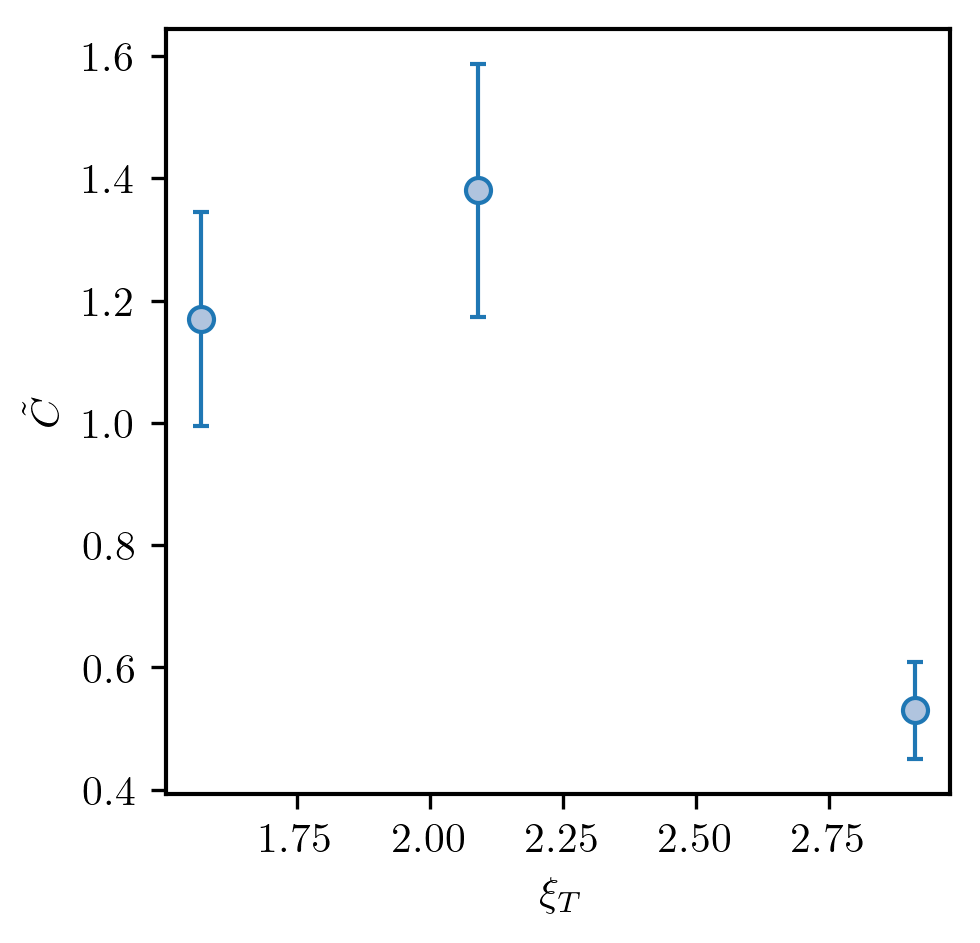
\includegraphics[width=0.6\textwidth]{Fig/Chapter5/C_tilde_vs_T.png}
    \caption[Rescaled contact $\tilde{C}$ as a function $\xi_T$ for a fixed $\xi_{\gamma}=0.113$]{Rescaled contact $\tilde{C}$ as a function $\xi_T$ for a fixed $\xi_{\gamma}=0.113$. The qualitative behavior is consistent with the predictions of \cite{yao2018tan} as $\tilde{C}$ decreases with $\lambda_T$. }
    \label{fig:C_tilde_vs_T}
\end{figure}

\subsection{Qualitative evolution with the interaction strength}

We plot on Fig.-\ref{fig:C_vs_N} the experimental bare contact $C$ as a function of $\bar{N}$ and the experimental rescaled contact $\tilde{C}$ as a function of $\xi_{\gamma}$ for a fixed temperature $T=0.8 \ \mu \rm{K}$ corresponding to $\xi_T=1.57$. Interestingly, $C$ and $\tilde{C}$ behave very differently: while $C$ increases by roughly an order of magnitude because of the dependency in $N^{5/2}$, $\tilde{C}$ is found to be close to constant. This is rather reassuring as we are able to observe strong variations of the bare experimental contact that nevertheless look to be qualitatively consistent with theory. According to Fig.-\ref{fig:C_theo}, $\tilde{C}$ should indeed be slowly increasing with $\xi_{\gamma}$ as we may observe here.

\begin{figure}
    \centering
    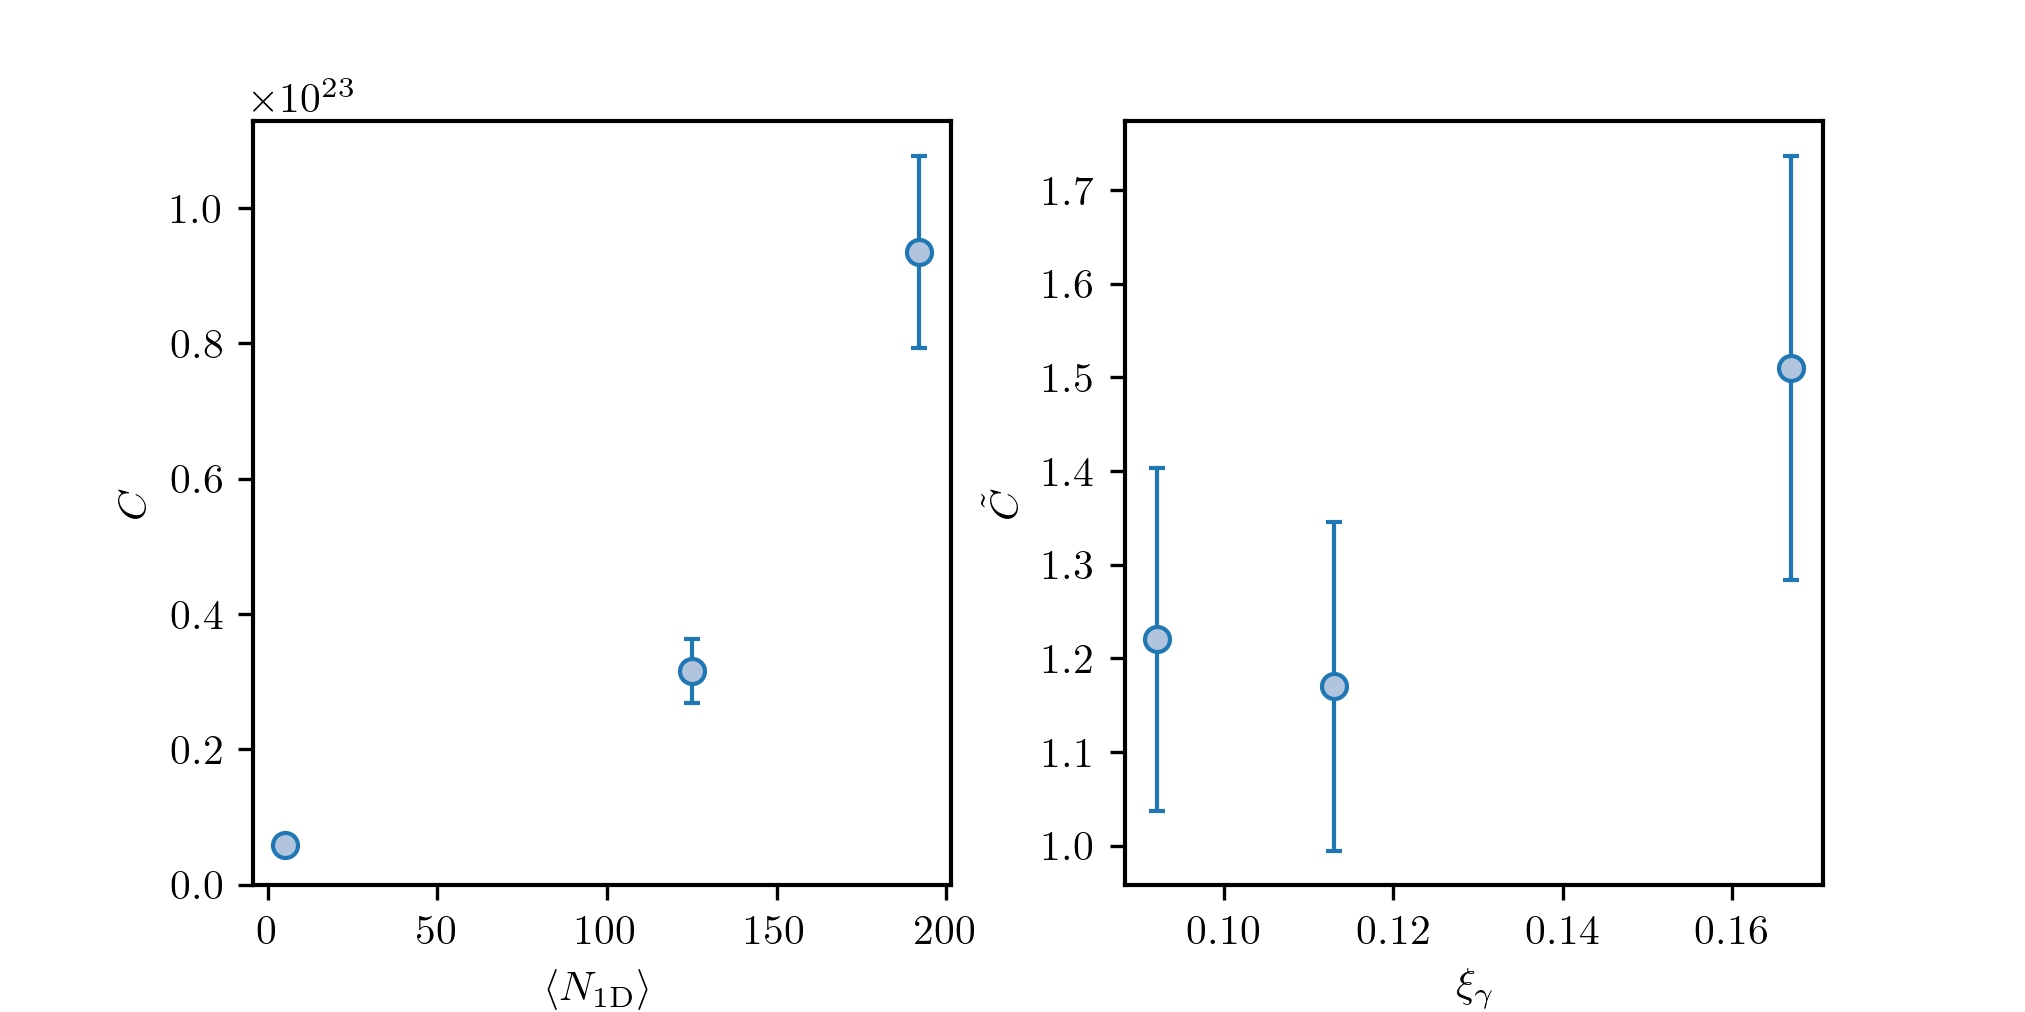
\includegraphics[width=\textwidth]{Fig/Chapter5/C_tilde_vs_N.png}
    \caption[Contact for various interaction strengths at a fixed temperature $\xi_T=1.57$]{Contact for various interaction strengths at a fixed temperature $\xi_T=1.57$ (a) Bare contact as a function of the weighted average number of atoms per tube $\bar{N}$. (b) Rescaled contact $\tilde{C}$ as a function of the reduced temperature $\xi_T$.}
    \label{fig:C_vs_N}
\end{figure}

\subsection{Comparison with QMC calculations}

So far, we have only discussed the qualitative evolution of $\tilde{C}$ with $\xi_T$ and $\xi_{\gamma}$ which seems encouraging and consistent with theory. We now push our study one step further by comparing the experimental data to {\it ab-initio} QMC calculations simulating our experiment. The calculations were once again performed by Hepeng Yao and simulate the distribution of tubes to match the experiment as precisely as possible. The results are plotted on Fig.-\ref{fig:1D_QMC_comparison} for two interaction parameters $\xi_{\gamma}=0.113$ and $\xi_{\gamma}=0.167$ corresponding to $\NBEC=1.1(1) \times 10^5$ and $\NBEC=3.1(3) \times 10^4$ for a fixed temperature $\xi_T=1.57$. The agreement for the low $k$ part is slightly off for the $\NBEC=1.1(1) \times 10^5$ data set, possibly due to a slight misevaluation of the temperature, but very good for the $\NBEC=3.1(3) \times 10^4$ data set, meaning that the method we use to describe the entire 2D array of 1D tubes and to determine the temperature is rather accurate, at least for low atom numbers. There is however a very clear disagreement by two orders of magnitude in the high $k$ part where the $\kmf$ tails are supposed to be.

\begin{figure}
    \centering
    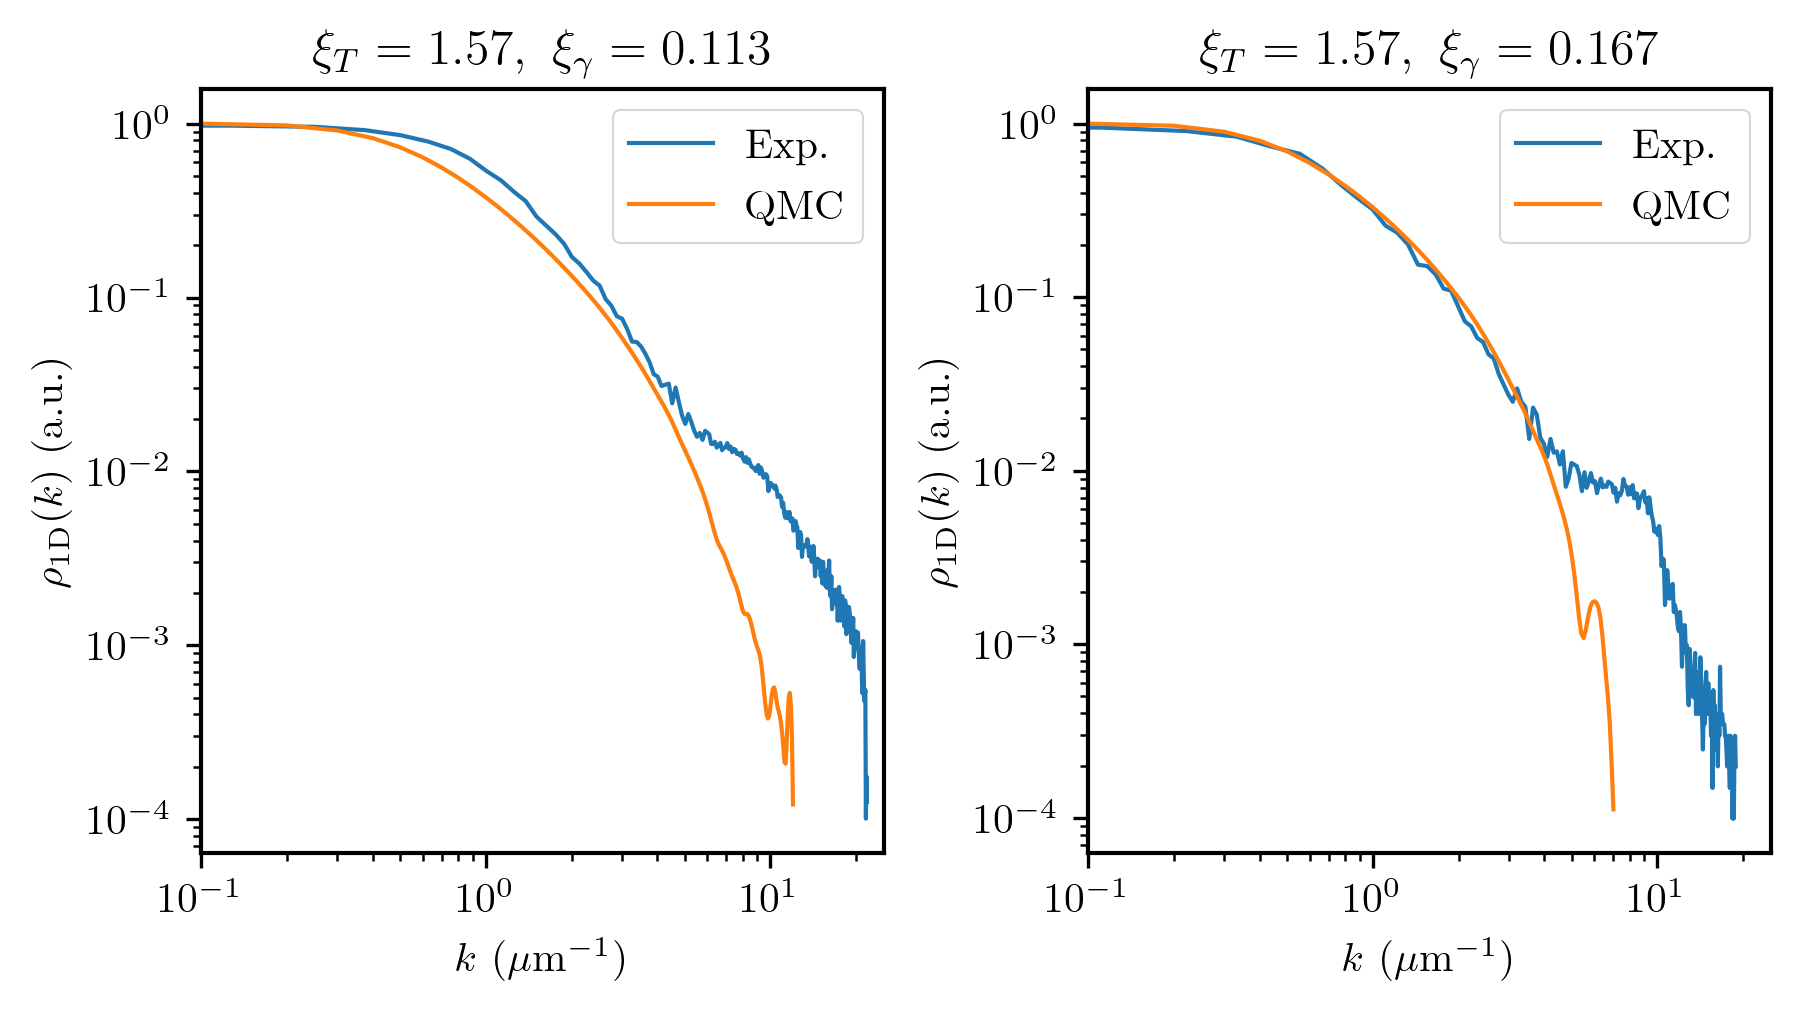
\includegraphics[width=0.9\textwidth]{Fig/Chapter5/QMC_comparison.png}
    \caption[Comparison between the normalized experimental data and QMC calculations for two different total atom numbers $\NBEC=110 \times 10^3$ and $\NBEC=31 \times 10^3$]{Comparison between the normalized experimental data and QMC calculations for two different total atom numbers $\NBEC=110 \times 10^3$ (left) and $\NBEC=31 \times 10^3$ (right).}
    \label{fig:1D_QMC_comparison}
\end{figure}

\subsubsection{Possible explanations}

It is actually not the first time that our team tried to measure a $\kmf$ scaling as we already attempted to measure this kind of scaling in the quantum depletion of a Bose-Einstein condensate. In \cite{chang2016momentum}, we actually measured a $\kmf$ scaling that was first attributed to Tan's contact but with too high of an amplitude, like in the case of the data presented here. Further investigations \cite{cayla_these} revealed that this scaling was in fact caused by $m_j=0$ impurities in the condensate that cannot be prevented from falling unto the MCP as they do not interact with magnetic fields. It was then the first hypothesis that we thought of to explain this discrepancy with the QMC calculations.

We then decided to characterize the effect of these $m_j=0$ atoms as well as the non-transferred $m_j=1$ that are not properly kicked that we will name ``background'' atoms by preparing the gases as we usually would and using the same displacement sequence, but not performing the population transfer in the beginning of the TOF. We performed a first test of the kind by preparing a gas with a deliberately low atom number $\NBEC=26(3) \times 10^3$, taking low and high momentum data as usual, and then measuring the distribution of $m_j=0$ for the same experimental sequence than used for the high momentum data. Even though the $m_j=0$ are unaffected by the magnetic field, we plot the distribution as if it were displaced to clearly compare it to the ``true'' displaced 1D distribution plotted in log-scale, as shown on Fig-\ref{fig:background_low_N}. We repeated this experiment for two different methods of removing the remaining non-transferred $m_j=1$ atoms, the first one being the usual method of using the $x$ gradient coil and the second one consisting in abruptly ramping up the current in the $y$ and $z$ bias coils to effectively create a gradient in time and push the atoms by doing so. We learn several things from these measurements:

\begin{itemize}
    \item The background density is higher when using the $y$ and $z$ bias coils than the $x$ gradient coil for the magnetic removal kick. This is rather reassuring has it had always been our preferred method so far. However, the shape of the two profiles are also slightly different. As these two data sets have been taken on the same day, this cannot be explained by day-to-day fluctuations of the state of the experiment. This could then mean that the $m_j=0$ atoms are not fully decoupled from the $m_j=1$ atoms during the TOF and that there could be some interactions affecting the shape of the background density. In addition, as the magnetic bias used to separate the magnetic sub-levels for the population transfer is along the $x$ direction, the kick using the $y$ and $z$ bias coils is not oriented along the quantification axis. This could result in some uncontrolled population transfer between the $m_j=1$ and the $m_j=0$ sub-states.
    \item The background density is however very close to the measured 1D distribution, especially with the $y,z$ removal kick where they overlap. Even worse, the background density seems to show a $\kmf$ decay as observed in the past.
    \item Contrary to the background density, the magnetic removal kick method does not affect the 1D momentum distribution. This could be explained using the argument stated earlier that using the $y$ and $z$ bias coils for the magnetic kick induces some population transfer from $m_j=1$ and $m_j=0$. While this effect is significant when no RF sweep population transfer  is performed, we can expect that it does not play any role when a large portion of the atoms have already been transferred to $m_j=0$ with the RF sweep.
    \item The plateau region that does not appear in the QMC data cannot however be explained by the effect of the background density which is roughly one order of magnitude lower in this momentum region.
\end{itemize}

\begin{figure}
    \centering
    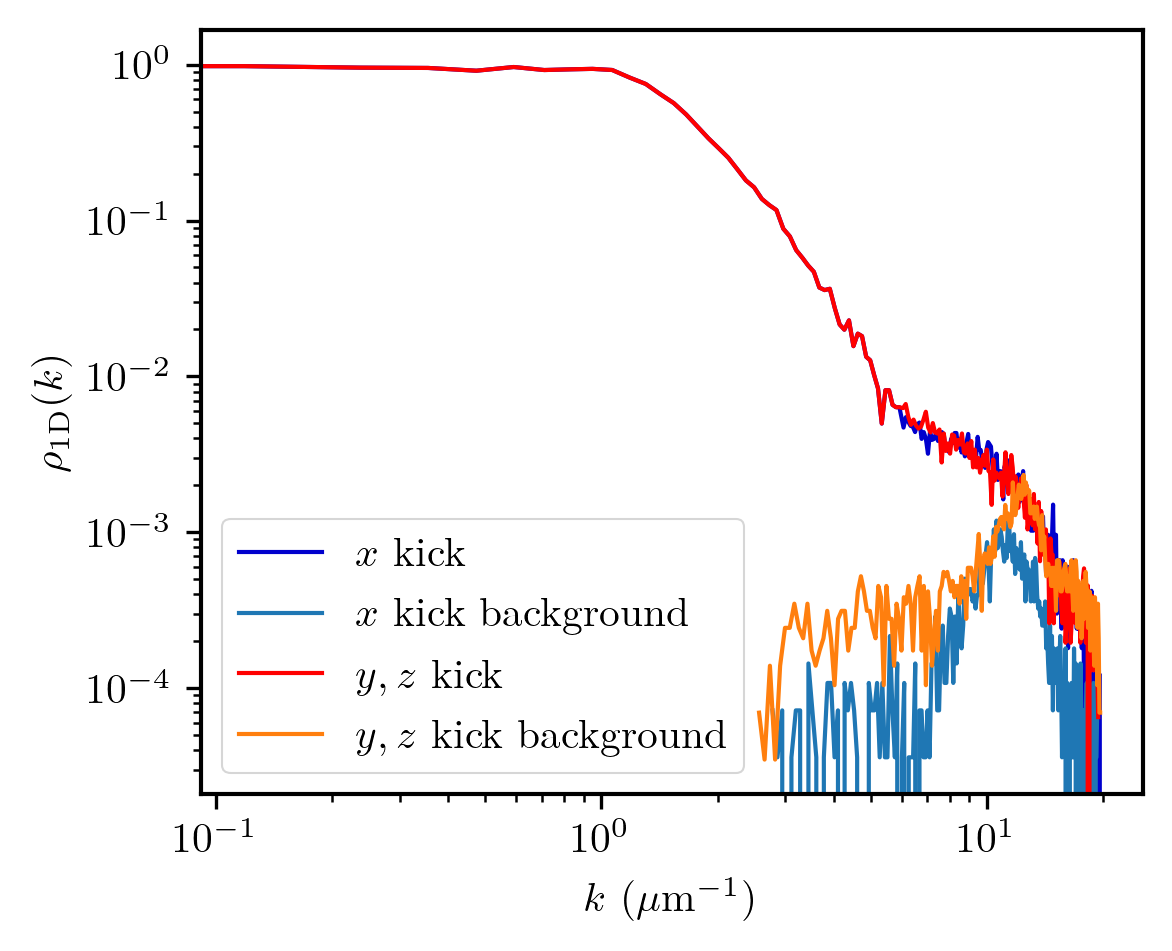
\includegraphics[width=0.7\textwidth]{Fig/Chapter5/1D_background_low.png}
    \caption[Effect of the background $m_j=0$ impurities for $\NBEC=26(3) \times 10^3$]{Effect of the background $m_j=0$ impurities for a total atom number $\NBEC=26(3) \times 10^3$. The experiment is done twice with two different methods of removing the non-transferred $m_j=1$ atoms in the beginning of the TOF, one using a gradient along $x$ (labelled as $x$ kick), one abruptly ramping up the current in the $y$ and $z$ bias coils (labelled as $y,z$ kick).}
    \label{fig:background_low_N}
\end{figure}

Unfortunately, these first tests seem to indicate that the $m_j=0$ impurities could indeed be playing a role, at least for low total atom numbers. We reproduced the same kind of experiment (this time leaving out the $y,z$ removal kick method) for a higher number of atoms $N = 1.1(1) \times 10^5$ with the results show in Fig-\ref{fig:background_high_N}. The data is strikingly different as the 1D density is about one order of magnitude higher than the background density in the $\kmf$ decay region! The $m_j=0$ impurities cannot then explain the discrepancy between the experimental and QMC data of the right panel of Fig-\ref{fig:1D_QMC_comparison} where the total atom number is similar.

\begin{figure}
    \centering
    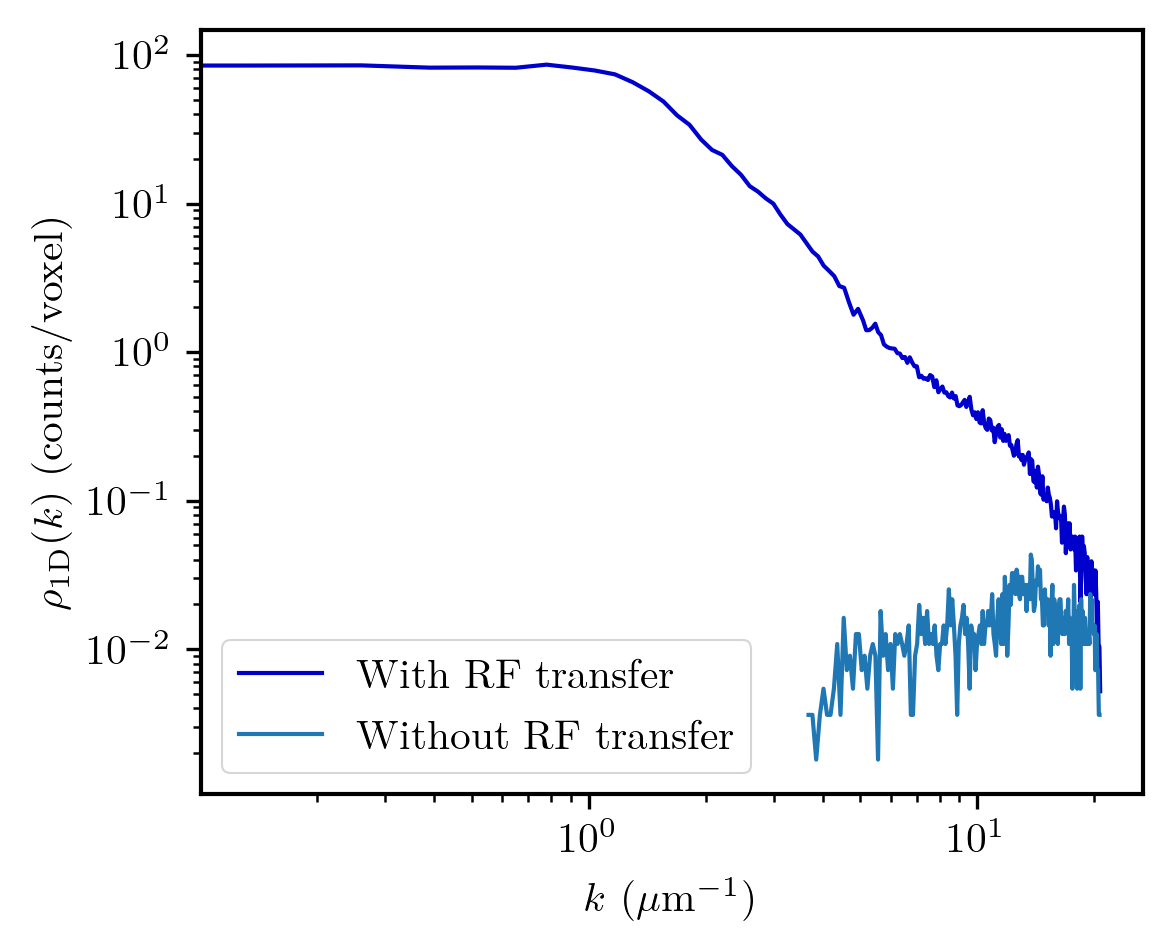
\includegraphics[width=0.7\textwidth]{Fig/Chapter5/1D_background_high.png}
    \caption[Effect of the background $m_j=0$ impurities for $\NBEC=1.1(1) \times 10^5$]{Effect of the background $m_j=0$ impurities for a total atom number $\NBEC=1.1(1) \times 10^5$}
    \label{fig:background_high_N}
\end{figure}

\section{Conclusion}

In conclusion, we observed qualitative behaviors of the amplitude of the $\kmf$ tails that seem to point towards the fact that we are measuring Tan's contact. However, the discrepancy with theory and QMC calculations is large and remains so far unexplained and an open question. While the first tests to quantify the effect of the $m_j=0$ impurities seem to indicate that they could partly explain the discrepancy at low atom numbers, this explanation does not hold for higher atom numbers. One of the principal questions to elucidate would be to understand what the intermediate algebraically decaying region means. We could indeed think that this is a physical feature related to the algebraic decay of the first order correlation function under the effect of interactions as explained in \ref{sec:1D_temperature}, but this is contradicted by the QMC calculations. We could however imagine that there is something that we did not properly understand in the way that the different 1D tubes contribute to the total distribution that the QMC calculations fail to reproduce. On the contrary, this could be the signature of some experimental defect that we have overlooked. 

In the near future, we plan to reproduce these experiments using the newly implemented two-photon Raman transfer. We hope that the increased detection efficiency will help us to separate more clearly the signal from the background effects and maybe help us identify more clearly what the problem sources are to find new paths to explore. 